\documentclass[a4paper]{article}

%% Language and font encodings
\usepackage[english]{babel}
\usepackage[utf8x]{inputenc}
\usepackage[T1]{fontenc}

%% Sets page size and margins
\usepackage[a4paper,top=3cm,bottom=2cm,left=3cm,right=3cm,marginparwidth=1.75cm]{geometry}

%% Useful packages
\usepackage{amsmath}
\usepackage{amssymb}
\usepackage{graphicx}
\usepackage[colorinlistoftodos]{todonotes}
\usepackage[colorlinks=true, allcolors=blue]{hyperref}
\usepackage{float}

\title{Cryogenic Buffer Gas Beam}
\author{Gary Chen}

\begin{document}
\maketitle

\section{Introduction}

We want to do stuff with ion-molecule chemistry and did it

\subsection{C$^+$ + H$_2$O Branching Ratio}

With our dual ablation system, we can reliably co-trap carbon and beryllium ions and introduce cold molecules from the CBGB. Introducing water entrained in a cold neon buffer gas beam, we can see the reaction products due to these collisions. Expected temperature of the buffer gas is 20K, which is defined by the temperature of the inner cell.

\subsubsection{Expected Reactions}

We do not expect any reactions to occur with the cold neon buffer gas. We have experimentally verified the absence of new mass peaks when introducing neon into the system with carbon and beryllium ions, only an overall loss rate attributed to elastic collisions within the trap.

Conversely, the water molecules will react readily with both beryllium and carbon ions:

\begin{align}
C^+ +H_2O & \rightarrow HCO^+ + H \label{r: HCO} \\
& \rightarrow COH^+ + H \label{r: COH} \\
Be^+ + H_2O & \rightarrow BeOH^+ + H  \label{r: beoh}
\end{align}

We want to probe the branching ratio of the formyl isomers formed in reactions \ref{r: HCO} and \ref{r: COH} at low temperatures. At room temperatures, the branching ratio has been found to be approximately 84:16 (HCO:COH)\cite{Freeman1987}, but unexplored at lower regimes. We have found that the total reaction rate of \ref{r: HCO}+\ref{r: COH} is approximately 2-3 times larger than that of \ref{r: beoh}, all reaction constants being around Langevin ($10^{-9} cm^3/s$).

To be able to find the branching ratio of the isomer products from reactions \ref{r: HCO} and \ref{r: COH}, we need to be able to separate their masses. 

Unfortunately, there are secondary reactions that also occur on the same time-scale, namely the reaction products from the initial reactions reacting with water again, which also happens around Langevin.

\begin{align}
HCO^+/COH^+ + H_2O &\rightarrow H_3O^+ + OH \label{r: c2}
\end{align}

\begin{table}
\centering
\caption{My caption}
\label{t: affinities}
\begin{tabular}{ll}
    & Affinity (kJ/mol) \\
COH & 427               \\
Kr  & 425               \\
HF  & 490               \\
N2  & 495               \\
Xe  & 496               \\
NO  & 531               \\
CO2 & 548               \\
CH4 & 552               \\
HCl & 564               \\
HBr & 569               \\
N2O & 571              
\end{tabular}
\end{table}

This poses a problem as we need to react away one of the isomers faster than they both become $H_3O^+$. Due to the fact that the hydrogen bond is on different molecules, each isomer has a different proton affinity as seen in table \ref{t: affinities} \cite{Love1987TheAffinity}

\subsection{Average Dipole Orientation Theory}

Adiabatic capture theory is a study of the long range potentials between particles to yield a collision cross section, which is then used to calculate a reaction rate constant. This is easily done for many potentials, such as the ion and induced-dipole interaction (Langevin), but is more difficult when considering potentials with another degree of freedom, in particular, we would like to consider the ion-dipole interaction. Unlike the Langevin interaction, the ion-dipole term has a angular term defined with respect to the inter-molecular axis. A few approximations are taken to give an average dipole orientation theory pioneered and expanded on by Su and Bowers.\cite{Su1973, Su1973a} This can also be extrapolated to include quadrupole interactions.\cite{Su1975}

\subsubsection{Standard Treatment}
A general method of calculating the rate constant of two particles with a given potential, blatantly taken from Willitch.\cite{Zhang2017} The attractive potential is a summation of interactions with coefficient $C_n$ and $r$ dependence $n$.

\begin{align}
    V(r) & = \sum_n -\frac{C_n}{r^n}
\end{align}

In the center of mass frame, we see that

\begin{align}
    V_{eff} & = \frac{l^2}{2 \mu r^2} - \sum_n \frac{C_n}{r^n}\label{eq: veff}
\end{align}

if $n > 2$, we can derive the capture cross section and rate constant as follows. First, we find the position $r_0$ corresponding to the maximum in the effective potential, which is the maximum of the centrifugal barrier.

\begin{align*}
    \frac{\partial V_{eff}(r_0)}{\partial r} & = 0 \\
    \therefore r_0 & = \left(\frac{n \mu, C_n}{l^2}\right)^{1/n-2}
\end{align*}

Substituting $r_0$ back into equation $\ref{eq: veff}$, we find the maximal value of the effective potential:

\begin{align}
    V_{eff}(r_0) & = \left(\frac{l^2}{\mu}\right)^{\frac{n}{n-2}} \frac{n-2}{2n}(n C_n)^{-\frac{2}{n-2}}
\end{align}

This then helps define the energy necessary for a collision, for if $E_{col}$ exceeds $V_{eff}(r_0)$, it will be able to surmount the barrier and react. Thus, we may define the maximum value for the angular momentum $l$ and the impact parameter $b$.

\begin{align*}
    l_{max} & = (\mu n)^{1/2}(C_n)^{1/n} \left(\frac{2 E_{col}}{n-2}\right)^{\frac{n-2}{2n}} \\
    b_{max} & = \frac{l_{max}}{\mu v}
\end{align*}

We can then define a collision cross section dependent on the collision energy:

\begin{align*}
    \sigma(E_{col}) & = \pi b^2_{max} \\
    & = \frac{\pi}{2} n \left(\frac{2}{n-2}\right)^{\frac{n-2}{2}} \left(\frac{C_n}{E_{col}}\right)^{\frac{2}{n}}
\end{align*}

Integrating the collision cross section with a Maxwell Boltzmann distribution yields a generalized rate constant as a function of temperature and n.

\begin{align}
    k(T) & = \int_0^{\infty} v f(v) \sigma(v) dv \label{eq: k int} \\
    & = \boxed{\sqrt{\frac{2 \pi}{\mu}}n\left(\frac{2}{n-2}\right)^{\frac{n-2}{2}}C_n^{2/n}(k_B T)^{\frac{n-4}{2n}}\Gamma\left(2-\frac{2}{n}\right)} \nonumber
\end{align}

\subsubsection{Ion-Dipole Interaction}

Langevin term of the ion and ion-induced dipole interaction:

\begin{align}
V_L(r)= &-\frac{\alpha q^2}{2r^4}
\end{align}

In the case of the ion-dipole interaction:

\begin{align}
V_D(r, \theta) = & -\frac{q\mu_D}{r^2} \cos(\theta)
\end{align}

The method outlined in section \ref{sec: langevin} finds the rate constant by dealing with a two body problem and only needing to consider the $r$ degree of freedom. The inclusion of the $\theta$ term complicates this, but to first order, we can parameterize it as a function of $r$. What we want to achieve is to write down the potential as such:

\begin{align}
    V(r) =& -\frac{\alpha q^2}{2r^4} - \frac{q\mu_D}{r^2} \cos\left(\bar{\theta}(r)\right) \nonumber \\
    \bar{\theta} = & \frac{\int \theta P(\theta) d\theta}{\int P(\theta) d\theta} \label{eq: avg theta}
\end{align}

Where $P(\theta)$ is the probability of finding the dipole at $\theta$. Two conditions arise:

\begin{enumerate}
\item $P(\theta)$ is inversely proportional to the angular velocity:
$$P(\theta) \propto 1/\dot{\theta}$$
\item An orientation has a probability weighted by the circumference of an angle:
$$C=2\pi l \sin(\theta)$$
$$ P(\theta) \propto \sin(\theta) $$
\end{enumerate}

So then the probability is a combination of the two situations:

\begin{align}
    P(\theta)=&\frac{\sin(\theta)}{\dot{\theta}} \label{eq: prob}
\end{align}

We can relate the angular velocity to the angular kinetic energy and the total energy in the system:
\begin{align}
    KE_{rot} & = \frac{1}{2}I\dot{\theta}^2 \nonumber \\
    E_{tot} & = KE_{rot} + V_D \label{eq: Etot}
\end{align}

Redefining equation \ref{eq: prob} with equation \ref{eq: Etot}, we find:
\begin{align}
    P(\theta) \propto & \frac{\sin(\theta)}{\sqrt{E_{rot}-V_D}} \label{eq: p theta}
\end{align}
%
Combining equations \ref{eq: p theta} and \ref{eq: avg theta} yields:

\begin{align}
    \bar{\theta} = & \frac{\int\frac{\theta \sin(\theta)d\theta}{\sqrt{E_{rot}+q\mu_D/r^2 \cos(\theta)}}}{\int\frac{\sin(\theta)d\theta}{\sqrt{E_{rot}+q\mu_D/r^2 \cos(\theta)}}} \label{eq: avg theta int}
\end{align}

From here, two situations arise:

\begin{enumerate}
\item $E_{rot} = E_1 < \frac{q \mu_D}{r^2}$
There is not enough rotational energy to overcome the dipole locking. The solution is oscillatory, but $\theta$ has a $r$ dependent bound. We let the maximal capture angle be defined as $K$.

$$ E_1=-\frac{q \mu_D}{r^2}\cos(K) $$

When substituted into equation \ref{eq: avg theta int}, we find:

\begin{align*}
    \bar{\theta}_1 & = \frac{\int_0^K \frac{\theta \sin(\theta) d \theta}{\sqrt{\cos(\theta) - \cos(K)}}}{\int_0^K \frac{\sin(\theta) d \theta}{\sqrt{\cos(\theta) - \cos(K)}}}
\end{align*}


After some math (something something integration by infinite series) and get a result of:

\begin{align*}
    \bar{\theta}_1 & = \frac{2 \sqrt{2}A}{\sqrt{1-\cos(K)}} \\
    \text{where }A & \equiv \int_0^{\pi/2} \frac{a^2 \cos(\phi)^2 d\phi}{\sqrt{q-a^2 \sin(\phi)^2}}
\end{align*}

\begin{figure}[H]
\label{fig: theta1}
\centering
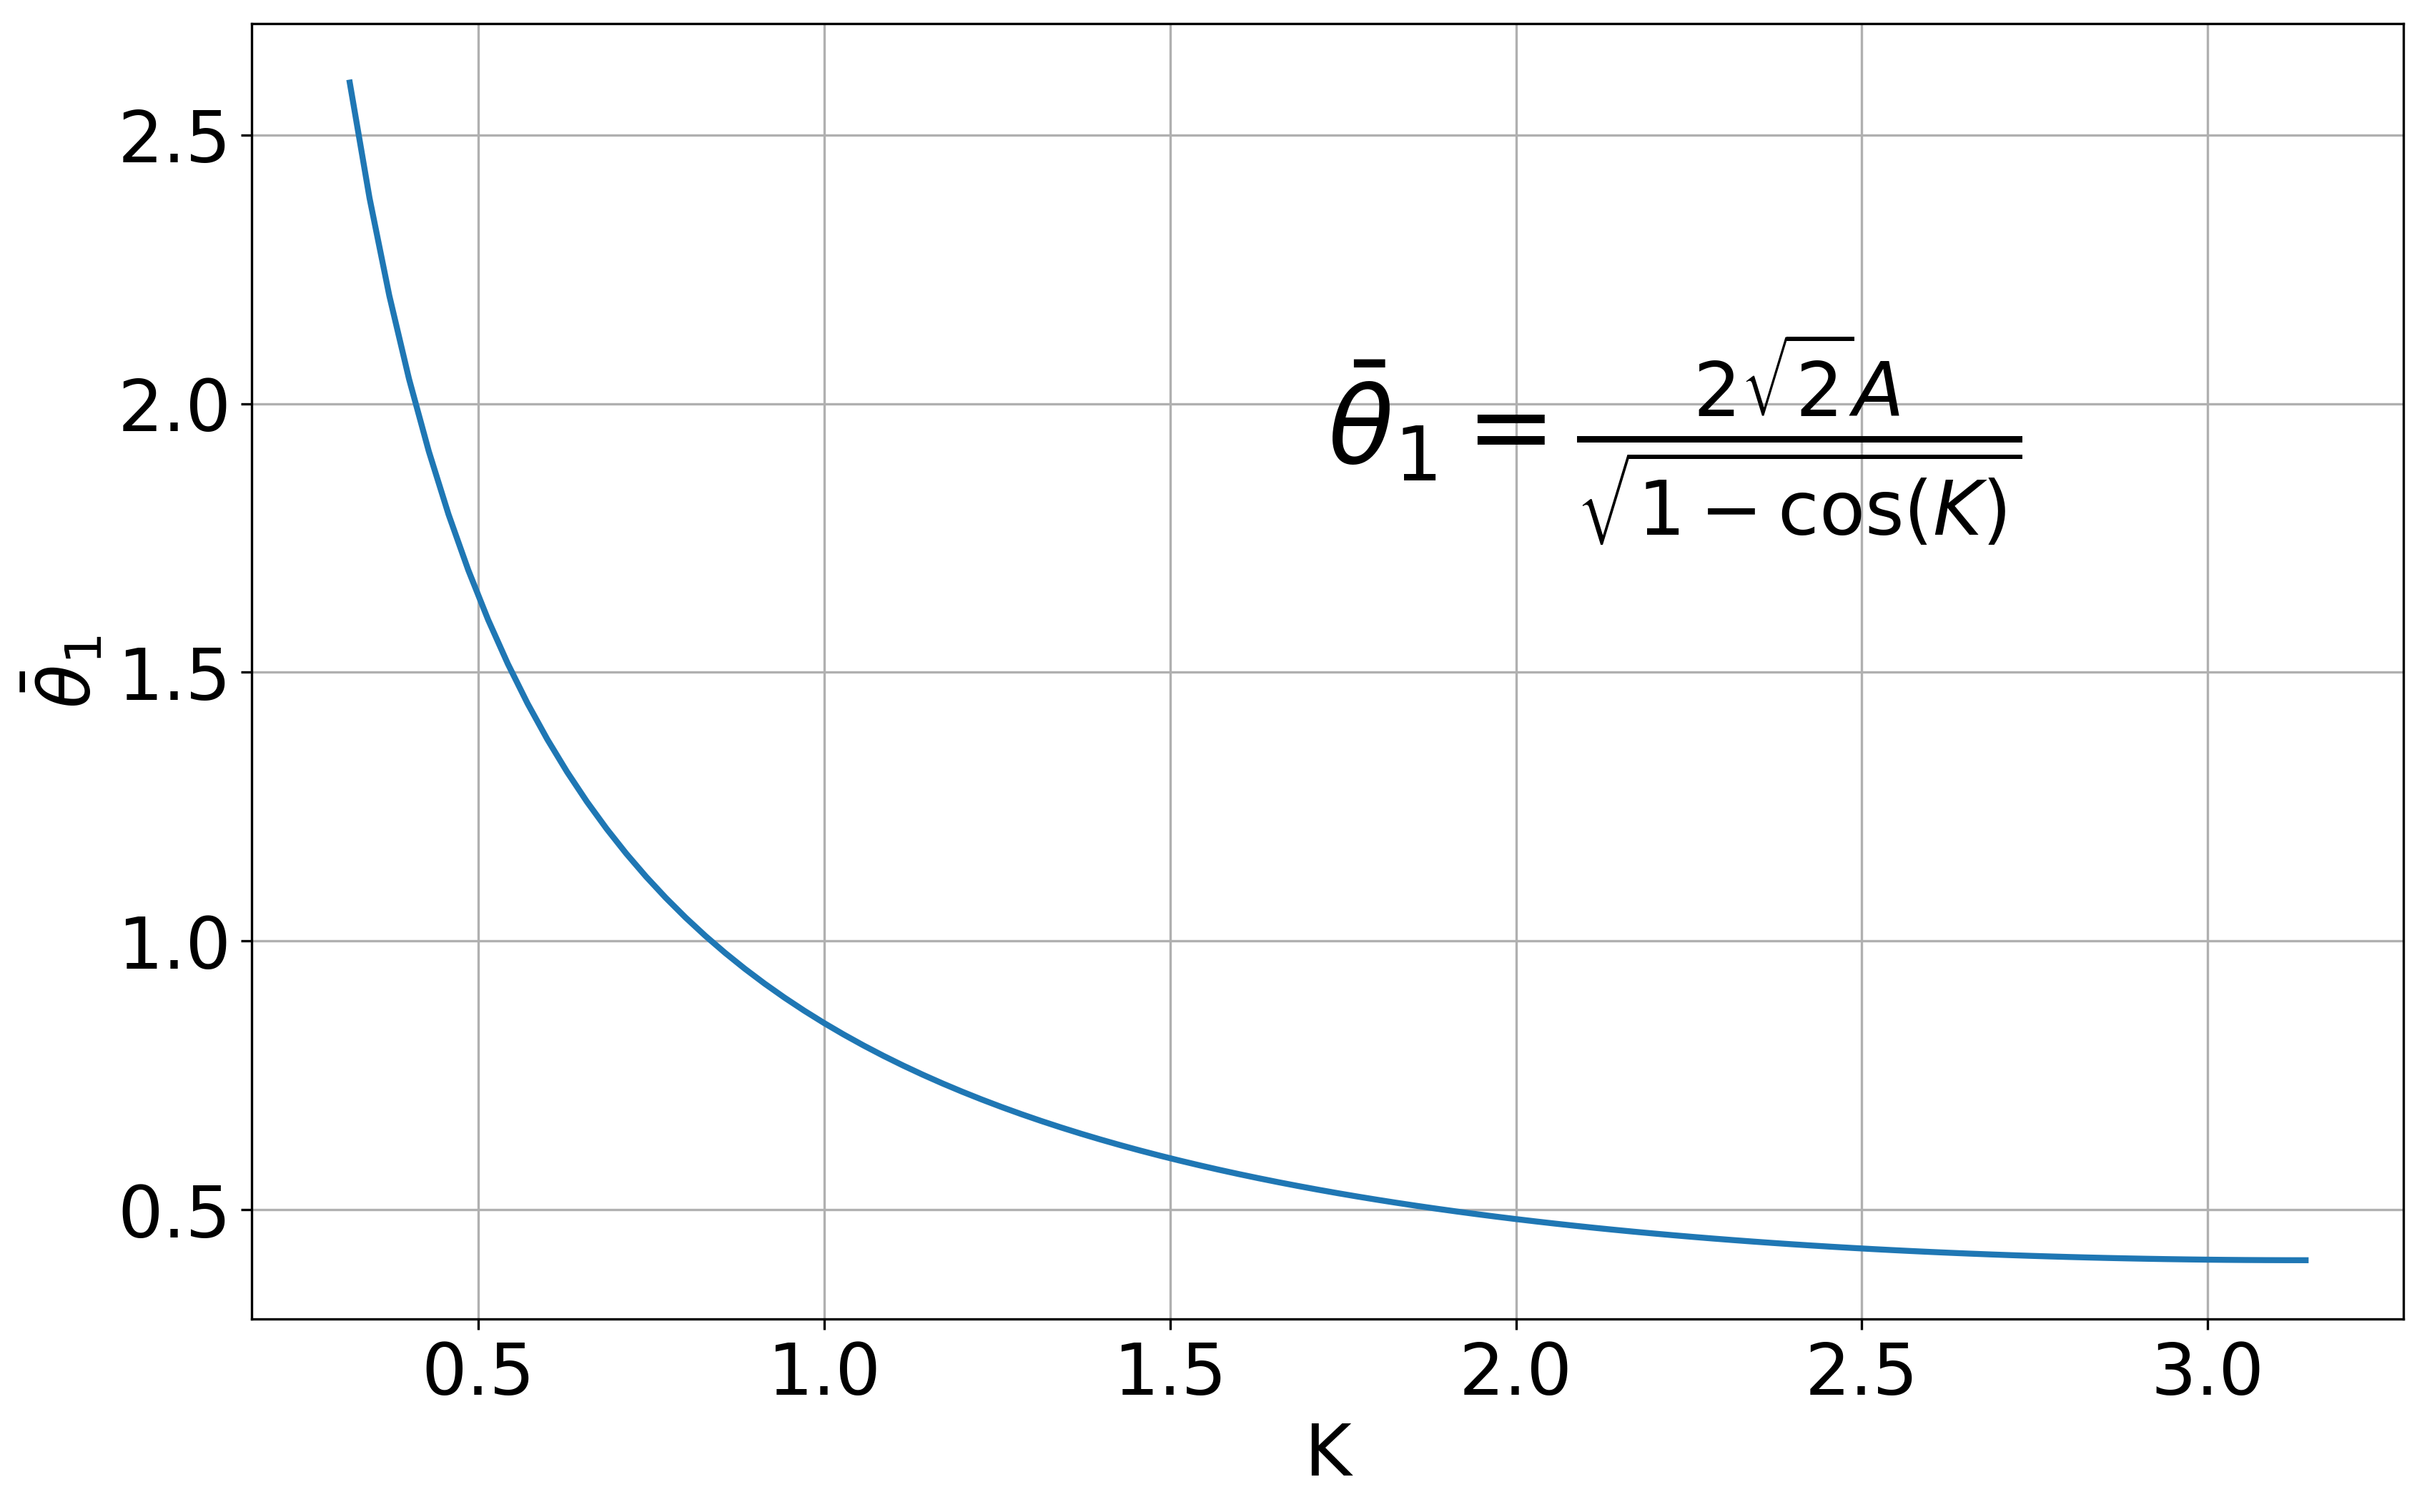
\includegraphics[width=0.8\textwidth]{ADO_theta1.png}
\caption{Rough plotting of $\theta_1$ as a function of maximum angle $K$. The behaviour is as expected, the greater the capture angle, the more $\theta_1$ tends towards 0.}
\end{figure}

\item $E_{rot} = E_1 > \frac{q \mu_D}{r^2}$
The rotational energy is enough to overcome the dipole locking and $\theta$ can swing around in a complete circle

\begin{align}
    \bar{\theta}_2 & = \frac{\int_0^\pi \frac{\theta \sin(\theta) d\theta}{\sqrt{E_2 + q \mu_D/r^2 \cos(\theta)}}}{\int_0^\pi \frac{\sin(\theta) d \theta}{\sqrt{E_2 + q \mu_D/r^2 \cos(\theta)}}}
\end{align}

This can be integrated numerically.
\begin{figure}[H]
\label{fig: theta2}
\centering
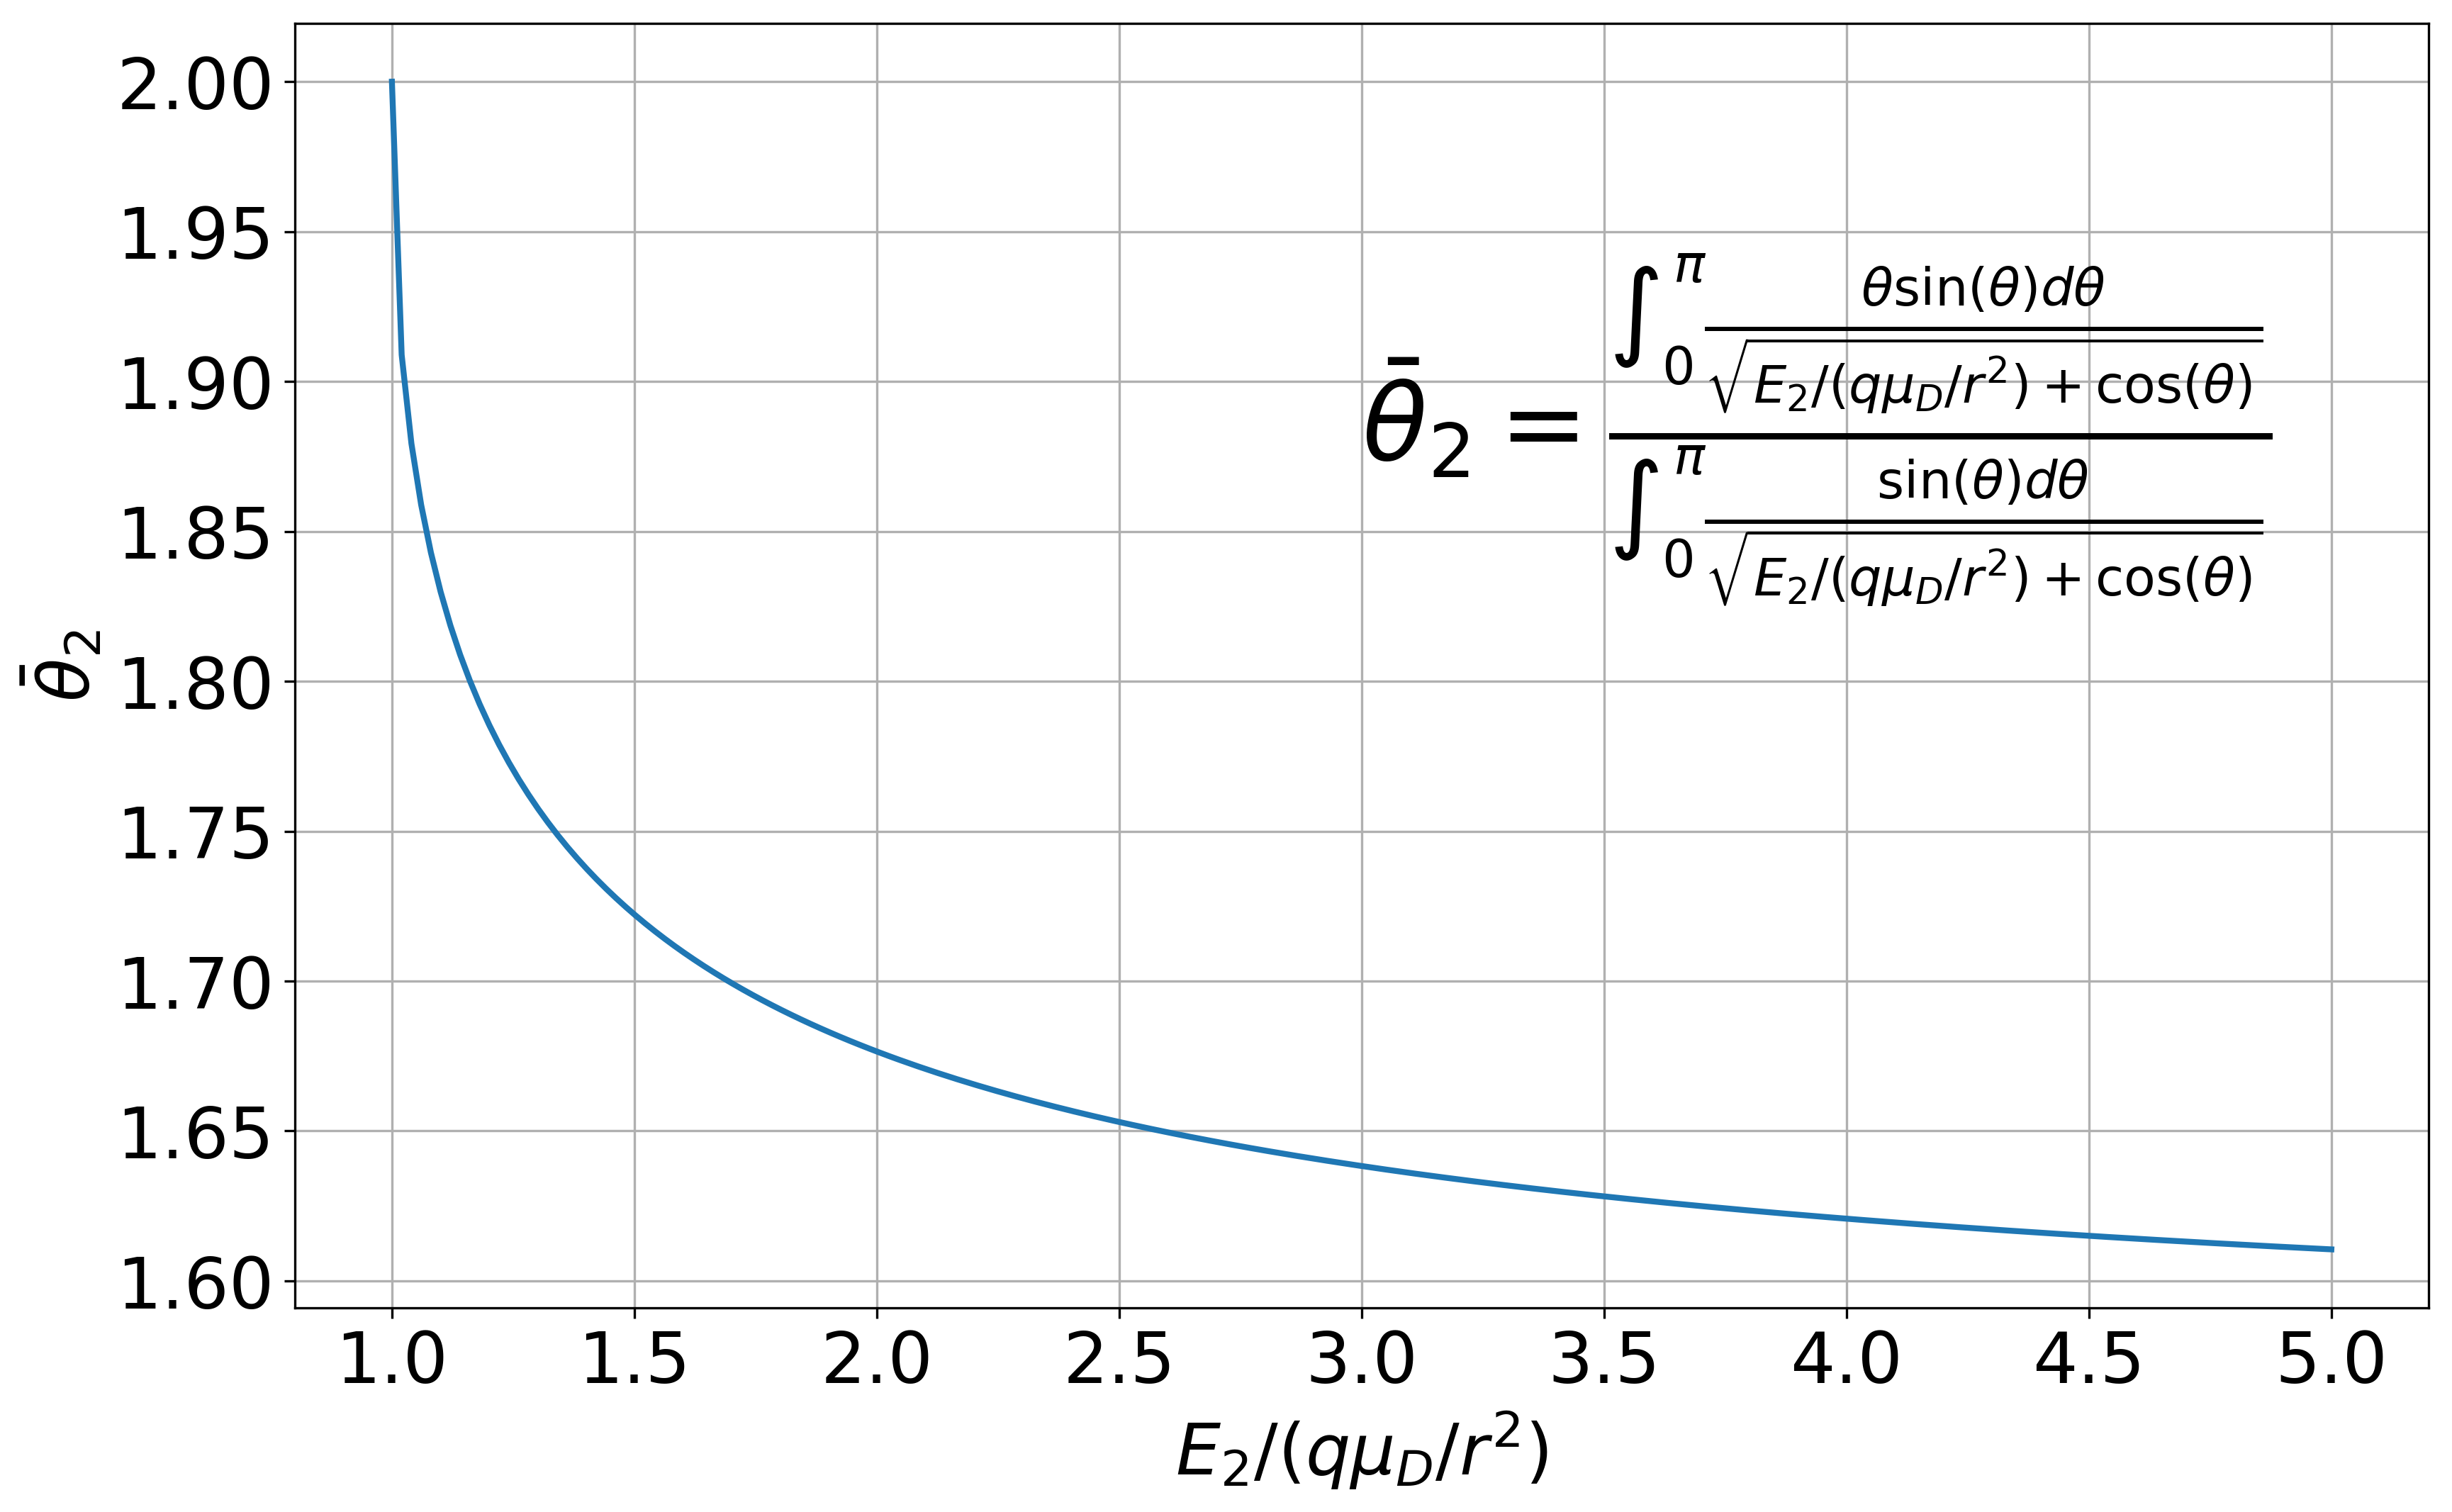
\includegraphics[width=0.8\textwidth]{ADO_theta2.png}
\caption{Rough plotting of $\theta_2$ as a function of the ratio of rotational energy and the monopole-dipole term. The low ratio behavior is not immediately obvious, but the greater the ratio between the rotational energy and monopole-dipole term, the more $\theta_2$ tends towards $\pi/2$ (sure).}
\end{figure}

\end{enumerate}

Let's say we have the forms for $\bar{\theta_1}$ and $\bar{\theta_2}$, we want to write down the full form of $\theta$. We can combine the two weighted by the probability of each as a function of internal energy.
\begin{align*}
    \bar{\theta}(r) & = \bar{\theta}_1(r) F_1 + \bar{\theta}_2(r) F_2
\end{align*}

Where these weightings are found via:

\begin{align*}
    P(\epsilon) d\epsilon & = \frac{1}{k_BT}e^{-\frac{\epsilon}{k_BT}}d\epsilon
\end{align*}

For diatomics, we can use:
\begin{align*}
    \epsilon & = \frac{J(J+1)\hbar^2}{2I}
\end{align*}

We can then use equation $\ref{eq: k int}$ and get a cross section and rate constant. The form is similar to that of just a Langevin term, but now with a dipole interaction term added onto it. All of the terms aside from $C$ come from the integration over the Boltzmann distribution, all of the angle averaging is wrapped up into the $C$ term.

\begin{align}
    k_{ADO} = & \frac{2 \pi e}{\sqrt{\mu}}\left(\sqrt{\alpha}+C \mu_D\sqrt{\frac{2}{\pi k_B T}}\right)
\end{align}

The dipole locking constant ($C$) can be numerically solved by iteratively integrating over combinations of $\mu_D$ and $\alpha$, or by looking at figure \ref{fig: C}.\cite{Su1973}\cite{Troe1985}

\begin{figure}[H]
\label{fig: C}
\centering
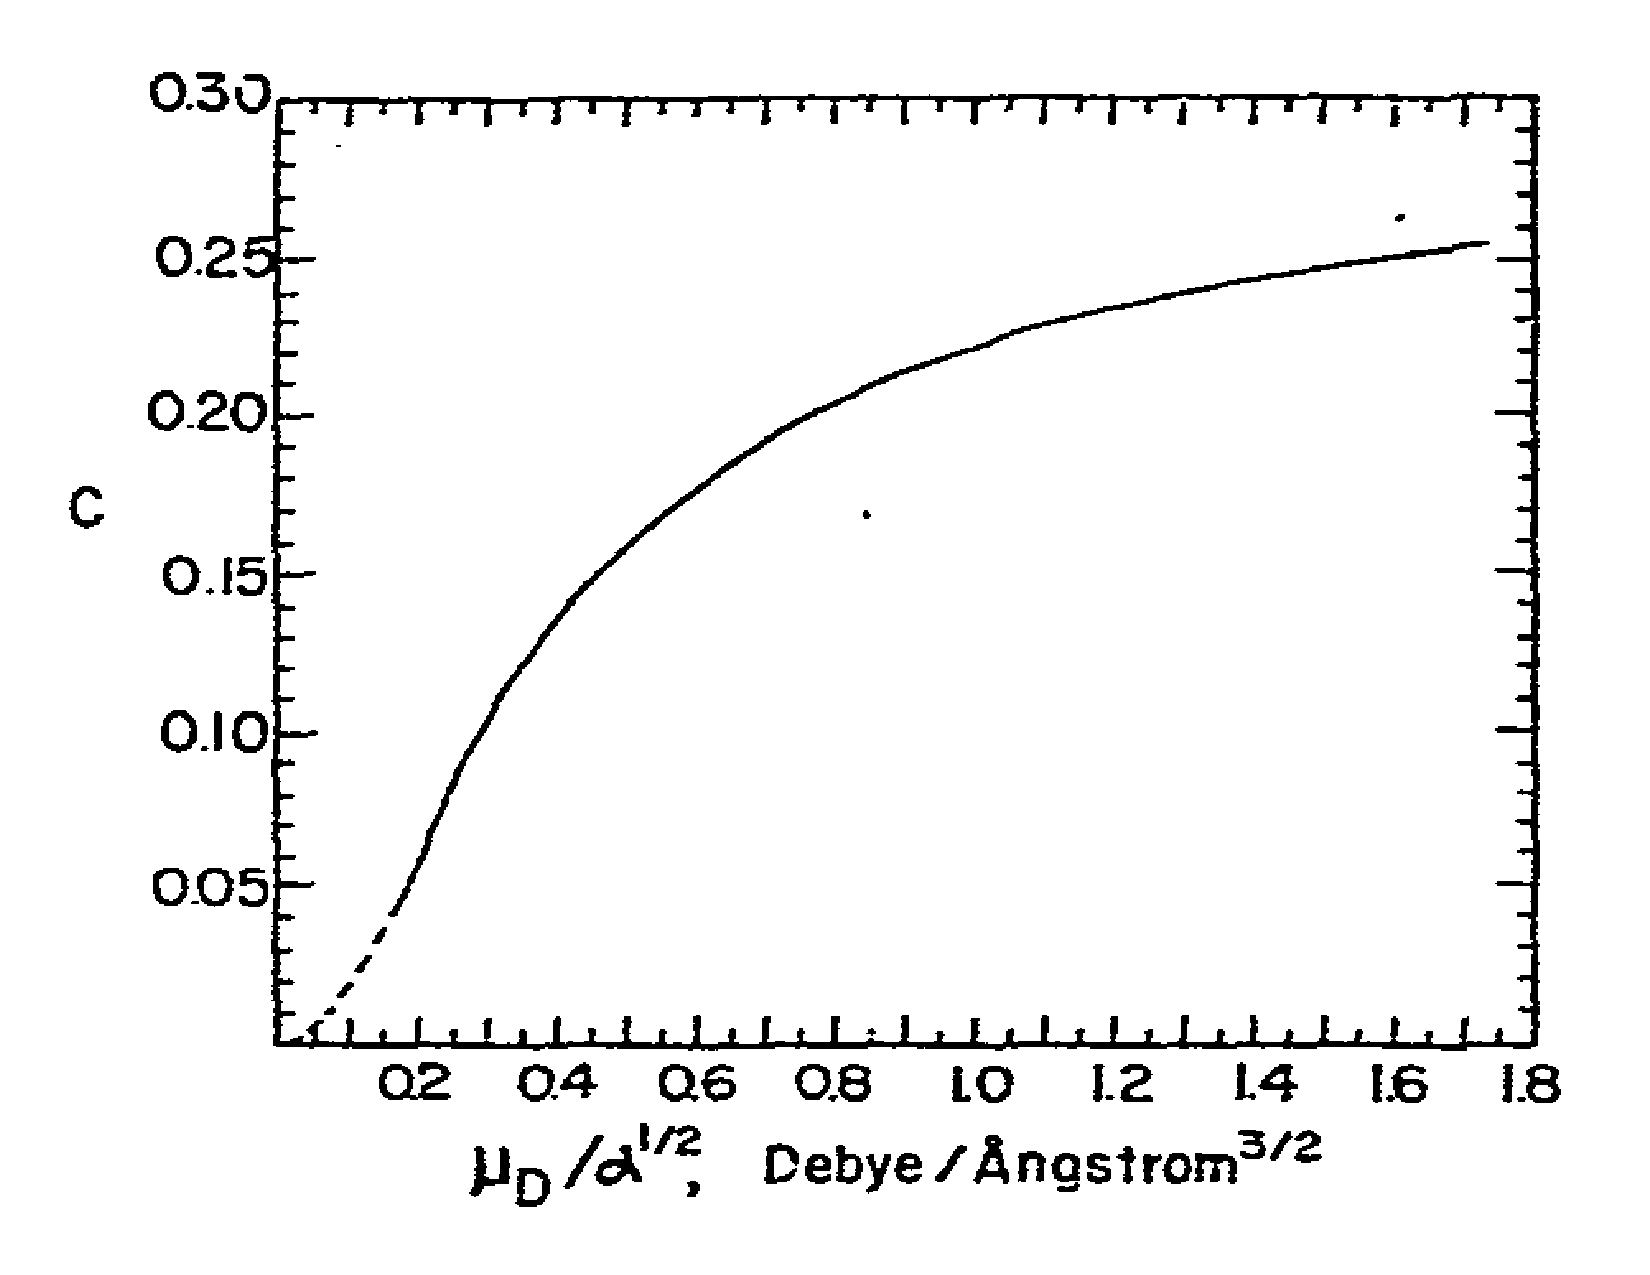
\includegraphics[width=0.8\textwidth]{ADO_C.pdf}
\caption{Dipole locking constant $C$ parameterized by the dipole moment $\mu_D$ and polarizability $\alpha$.\cite{Su1973}}
\end{figure}

\subsection{Introduction to Buffer Gas Beams}

To reach reaction temperatures in the regime of 10K from a beam of molecules with trapped ions, a cryogenic buffer gas beam (CBGB) of neon with entrained water is employed. Numerous methods of creating cold beams of molecules exist, from Zeeman decelerators \cite{Narevicius2008}, Stark decelerators, to cryogenic buffer gas beams (CBGB). CBGB's in particular have the benefit of being species agnostic, where the resultant beam properties are not dependent on the target species at hand, rather, the buffer gas species. \todo{Add citations for decelerators}

By holding a cell filled with a buffer gas of neon of helium above its vapor pressure, a volume of gas can be held at cryogenic temperatures. Other species of molecules are atoms may be introduced into the buffer gas cell via ablation, fill line, etc. The target species particles are then sympathetically cooled via collisions with the cold buffer gas. An aperture at one end of the cell allows for the extraction of the buffer gas and entrained target species into a beam. Regulating the buffer gas cell temperature to above 17K for neon, and 4K for helium, in high vacuum allows us to accumulate an appreciable stagnation number density.
\todo{Add graphic to show what a buffer gas beam is}

The Reynolds number is typically used to characterize the flow regime of the buffer gas beam. At the aperture of the buffer gas cell, the Reynolds number can be written as:

\begin{align} \label{e: reynolds}
Re & \approx \frac{2 d_{aperture}}{\lambda} \\
& \approx \frac{8\sqrt[]{2} \dot{N} \sigma}{d_{aperture} \bar{v}}
\end{align}

Where $d_{aperture}$ is the diameter of the aperture and $\lambda$ is the mean free path of the buffer gas particles \cite{Hutzler2012}.

\subsubsection{Beam Velocity}

At thermal equilibrium, the velocities inside the buffer gas cell follows a Maxwell Boltzmann distribution:

\begin{align} \label{e: mb_distribution}
f(v) & = \left(\frac{m}{2 \pi k T}\right)^{3/2}4 \pi v^2 e^{-\frac{m v^2}{2 k T}}
\end{align}

Where the mean velocity is:

\begin{align} \label{e: mb_mean}
\bar{v} & = \sqrt{\frac{8 k_B T}{\pi m}}
\end{align}

We may rewrite the distribution as a function of the mean velocity $\bar{v}$ into a simpler form .

\begin{align} \label{e: mb_simplified}
f(v) & = \frac{32}{\pi^2} \frac{v^2}{\bar{v}^3} e^{-4v^2/\pi \bar{v}^2}
\end{align}

To get the velocity distribution in the beam, we can calculate the distribution of particles incident on an aperture in the cell.

\begin{align}
f_{beam}(v) & = \frac{v}{\bar{v}}f(v)  \\
& = \frac{32}{\pi^2} \frac{v^3}{\bar{v}^4} e^{-4v^2/\pi \bar{v}^2}
\end{align}

For low Reynold's numbers (Re<1) the flow at the aperture is purely molecular, which means that there are few to no collisions. This allows us to continue to use the Maxwell-Boltzmann distribution to describe the forward velocity \cite{Hutzler2011c}.

\begin{align}
\bar{v}_\parallel & = \int_0^\infty v f(v) dv \approx 1.2 \bar{v}
\end{align}

The spread of the forward velocity of an effusive beam is the full width half max (FWHM) of the Maxwell-Boltzmann distribution: $\Delta\bar{v} \approx 1.5 \bar{v}$.

As one increases the Reynolds number, one can reach the supersonic regime (Re>100) where the velocity reaches $1.4\bar{v}$ \cite{Hutzler2011c}.

But as the flow regime nears the supersonic regime, forward collisions around the aperture cause boosting of the average velocity as well as a decrease in the velocity spread. Changing the flow regime may also change the ratio of species in the beam as well.

A helium buffer gas held at 4K will be slower than a neon gas held at 17K. Despite this, it is preferable to use neon as a buffer gas due to its ideal cryopumping properties. Helium requires large amounts of activated charcoal, also held at low temperatures, to effectively cryopump. These volumes of charcoal can then become saturated and require purging, limiting one's operating time. Neon on the other hand, only requires a metal surface lower than 17K to create neon ice. The neon ice surface will then act as a cryopump for more neon gas as well, allowing for hours of continuous operation with no appreciable build up of background gas. Our experiment uses neon as a buffer gas for its technical simplicity, the lower achievable temperature with the helium does not yield dramatic gains in the final reaction temperature.

\subsubsection{Density and Extraction}

The stagnation density inside the buffer gas cell is a function of the physical dimensions of the cell and the number flow rate into the cell. High stagnation densities allows for high densities of reactants at the ion trap center, but can push the beam into an unwanted flow regime where the beam properties are not what one wants. Experimentally, it's preferable to use volumetric flow rates when operating the apparatus, but for calculations, that needs to translate to number flow rate using the ideal gas law:

\begin{align}
\dot{N} = \frac{P f}{k_B T}
\end{align}

where $P$ is pressure and $f$ is the volumetric flow rate, this translates to about $4\times10^{17} \text{ particles} \cdot \text{s}^{-1}$ for 1 SCCM of gas flow. By solving for the number density in the flow out of an aperture with molecular flow, we find that the stagnation density within the cell can be shown as:

\begin{align}
n_{b}=\frac{4 \dot{N}}{A_{aperture} \bar{v}}
\end{align}

In general, buffer gas beams operate with stagnation densities around $10^{15}-10^{17} cm^{-3}$. Outside of the cell, we can describe the density of the beam as a function of distance. \cite{Pauly}

\begin{align}
n(z)=\frac{n_o}{2}\left(1-\frac{z}{\sqrt{z^2+a^2}}\right)
\end{align}

Where $z$ is the distance from the aperture into the vacuum side, $n_o$ is the initial number density, $a$ is the radius of the aperture. In the far field, this goes to

\begin{align}
n(z)=\frac{n_o a^2}{4 z^2}
\end{align}

But there is something that we must consider, that is that we aren't seeing the full aperture while we are at all locations, we are actually seeing an appended area due to the inclusion of apertures and skimmers in the way. So in the calculation for $n(z)$, only $n_o$ has a dependence on the aperture size of the cell, $n(z)$ itself will have a set value defined by the smallest aperture in the beam path.

Sympathetic cooling occurs through collisions between the hot target species being introduced and the cryogenic buffer gas particles. The thermalization of the target species with the buffer gas particles is derived via momentum conservation of hard sphere collisions, where $\approx 10$ and $\approx 100$ collisions are needed to relax translational and rotational states to within a factor of 2 of the buffer gas temperature. Vibrational degrees of freedom may take upwards of $10^4$ collisions to fully thermalize is the elastic collision energy is much lower than the internal vibrational level. By finding the mean free path, we can consider the characteristic length the particles travel to be thermalized with the buffer gas, this is then compared to the characteristic length of the cell to determine the effectiveness of the cooling.

\begin{align}
\lambda = \frac{A_{aperture} \bar{v}}{4 f \sigma \sqrt{m_s/m_b}}
\end{align}

If a species is introduced into the buffer gas cell that has a lower vapor pressure than that is allowed at the current temperature, it will be lost when it comes in contact with the cell walls. The rate of this loss can be described as the  characteristic time of diffusion of a particle in the buffer gas to the physical dimensions of the cell set the diffusion time constant:

\begin{align}
\tau_{diff} = \frac{16}{9 \pi} \frac{A_{cell} n_{0,b} \sigma}{\bar{v}}
\end{align}

where $\sigma$ represents the collisional cross section for the buffer gas with the target species. On the other hand, we have the characteristic pump out time given by the conductance of a cell aperture:

\begin{align}
\tau_{pump}=\frac{4V_{cell}}{\bar{v}A_{aperture}}
\end{align}

By combining the $\tau_{diff}$ with the $\tau_{pump}$, we can get a dimensionless ratio, $\gamma$ that characterizes the extraction fraction out of the cell.

\begin{align}
\gamma = \frac{\tau_{diff}}{\tau_{pump}} = \frac{\sigma f}{L_{cell} \bar{v}} \label{e: gamma}
\end{align}

Notice that the $\gamma$ factor does not depend on aperture size, this is generally true, but increasing the aperture size will lower your number density within the cell, which then influences the characteristic length scale of thermalization. Larger apertures thus run the risk of not allowing your particles to fully thermalize in rotational/vibrational states. But decreasing the aperture size can make alignment as well as controlling the number density more difficult, as finer control over the flow rate is necessary for equivalent flow regimes.

\section{Experimental Apparatus}
\subsection{Ion Trap}

\subsection{Cryogenic Buffer Gas Beam}

The CBGB apparatus was homebuilt out of aluminum for the outer chamber as well as the inner 40K radiation shield. A Cryomech PT415 Pulse Tube Refrigerator with a remote head option was inserted into the chamber. A large bellows attachment connected the pulse tube cooler head to the chamber itself to isolate the chamber from the mechanical vibrations caused by the pulse tube cooler itself.

The pulse tube cooler itself has 2 cooling stages and a room temperature stage. The room temperature stage at the top is where 

\begin{figure}[H]
\centering
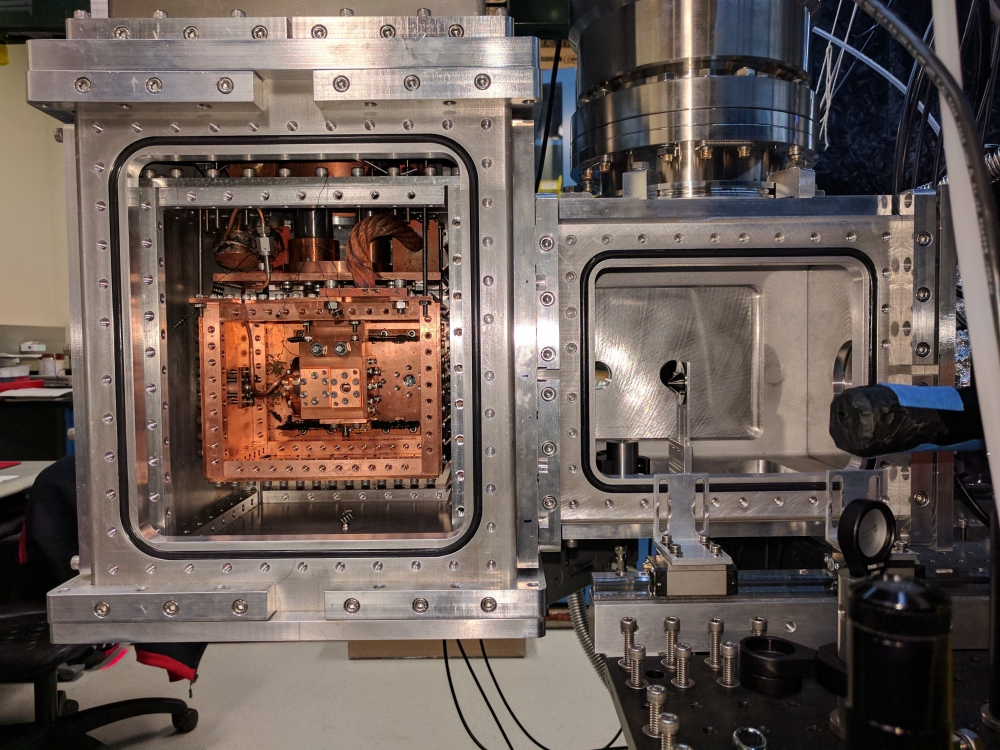
\includegraphics[width=1\textwidth]{apparatus_cross_section.jpg}
\caption{Cross sectional view of CBGB with side walls removed from the outer vacuum chamber, 40K aluminum radiation shield, and inner 4K cryopumping shield.}
\label{f: chamber}
\end{figure}

\begin{figure}[H]
\centering
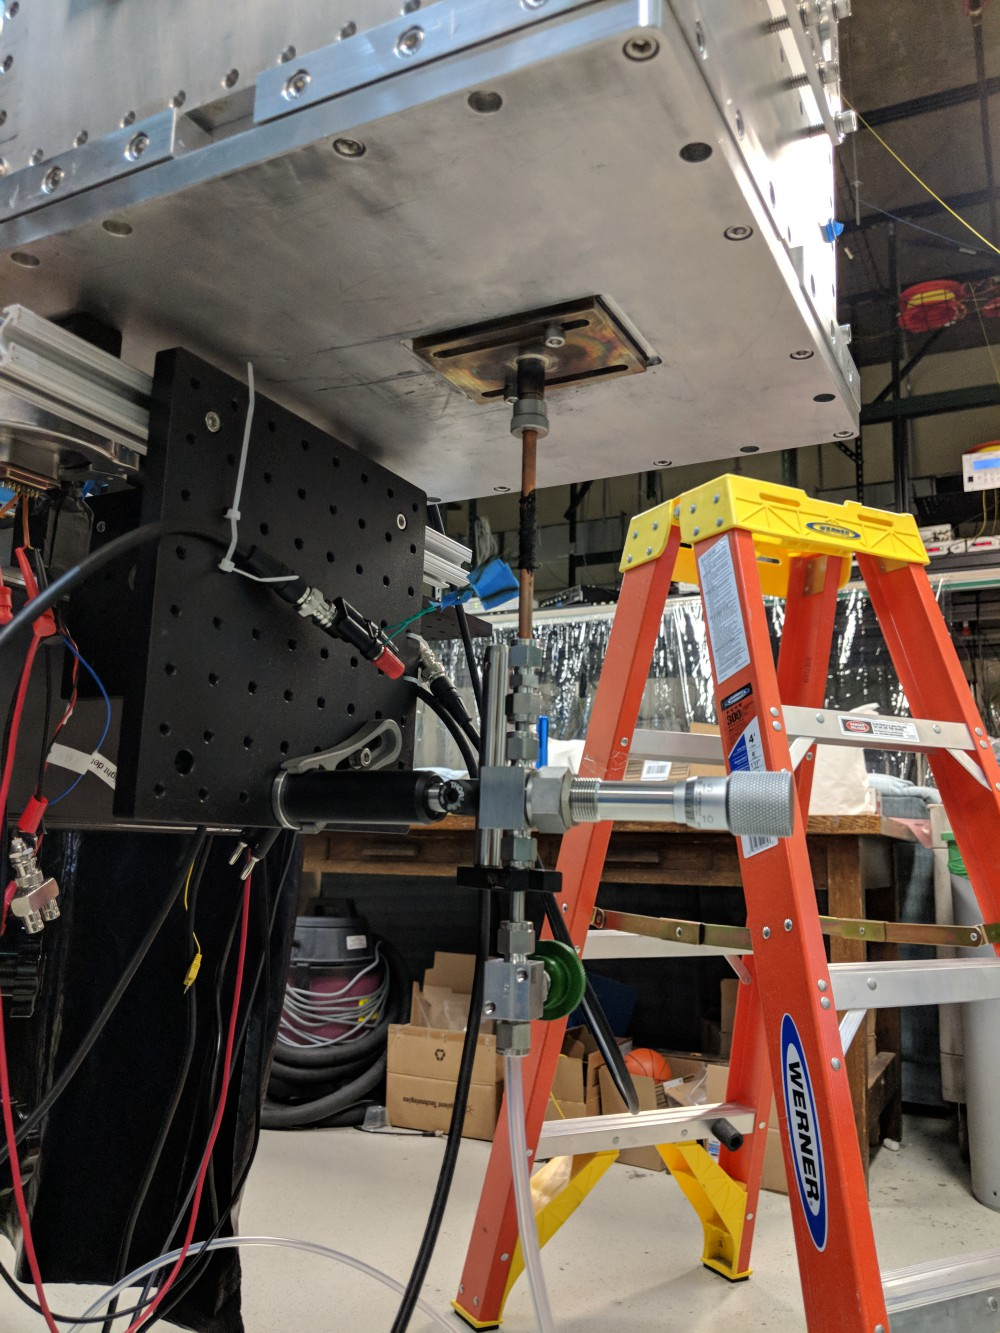
\includegraphics[width=.7\textwidth]{apparatus_water_fill_outside.jpg}
\caption{The water fill line, sealed by an ultratorr fitting and heated by nichrome wire. A shut off valve and vernier valve are used to regulate the flow of water into the buffer gas cell.}
\label{f: outside}
\end{figure}

\begin{figure}[H]
\centering
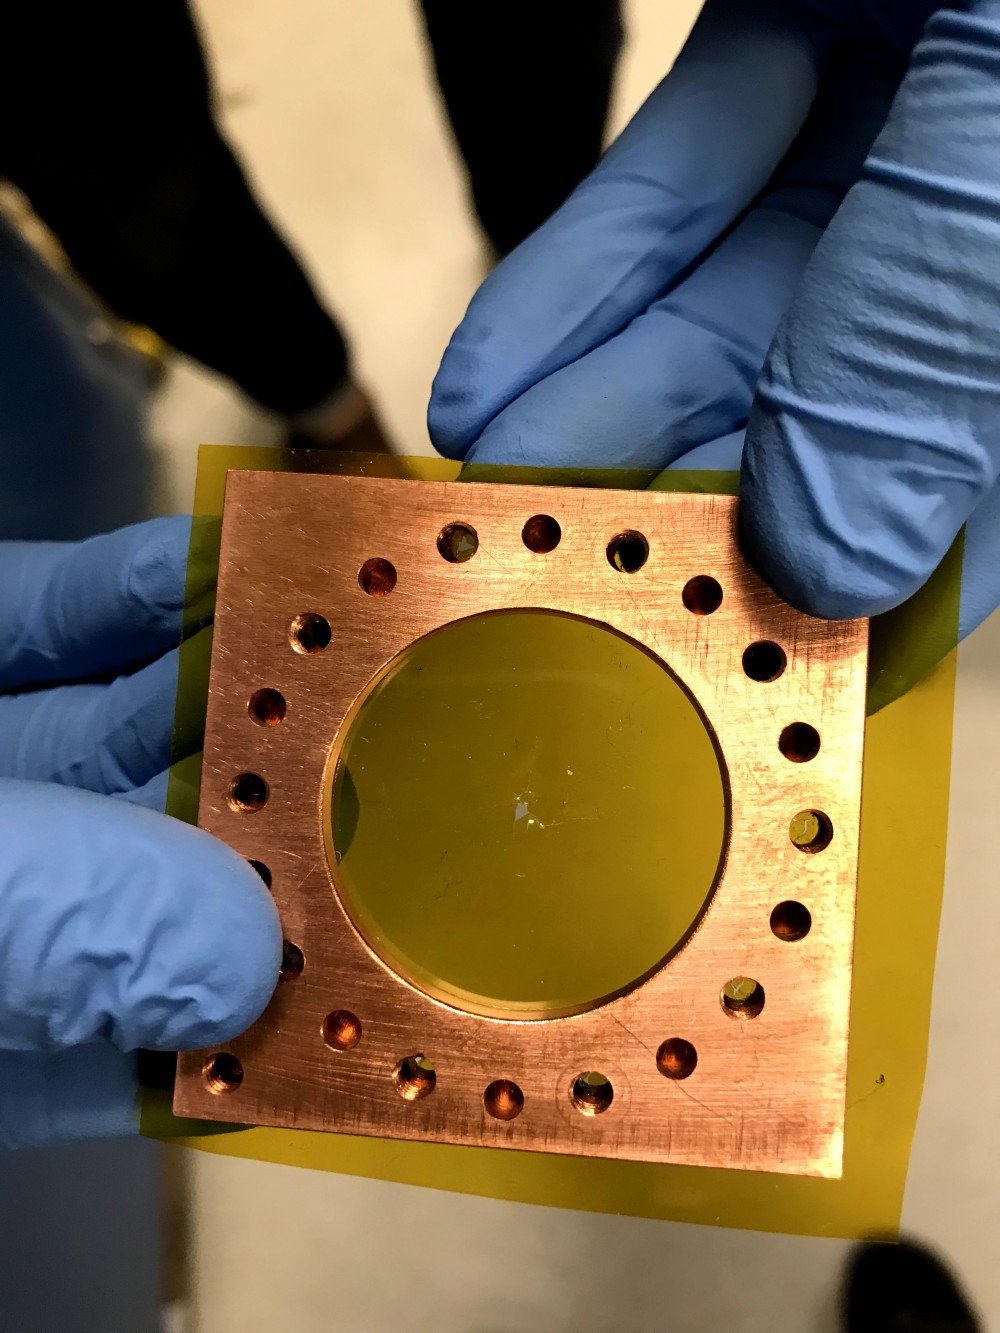
\includegraphics[width=.7\textwidth]{apparatus_kapton.jpg}
\caption{A kapton film serves as the back wall of the buffer gas cell with a hole for the insertion of the water fill line. The kapton surface resists ice formation and allows for continuous operation with water for over 10 hours.}
\label{f: kapton}
\end{figure}

\begin{figure} [H]
\centering
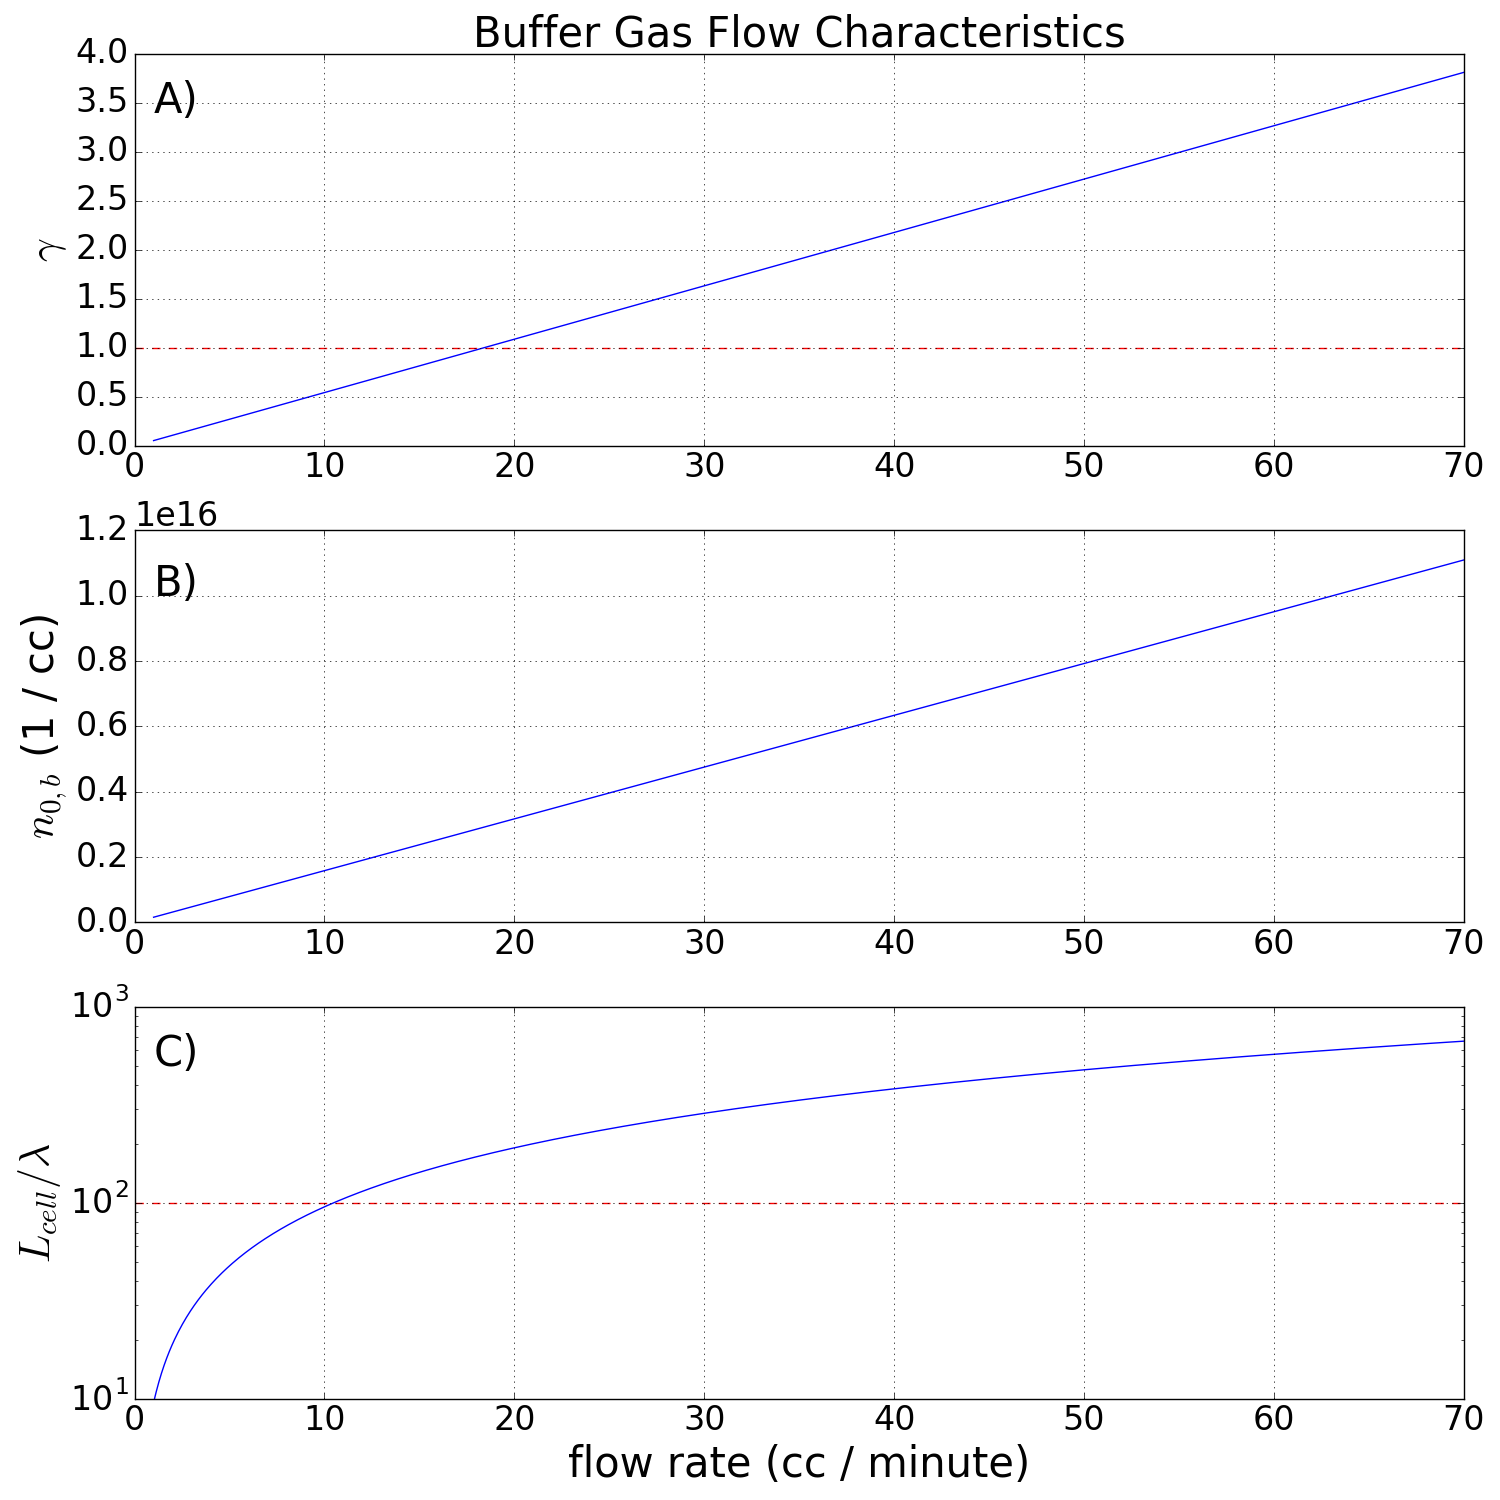
\includegraphics[width=1\textwidth]{CBGB_flow_characteristic.png}
\caption{A) $\gamma$ extraction ratio, dotted red line indicates $\gamma = 1$ where hydrodynamic entrainment begins. B) Theoretical number density of buffer gas species within buffer gas cell. C) Number of collisions one would expect before extraction out of the cell, dotted red line indicates 100 collisions before extraction when rotational degrees of freedom should be thermalized.}
\label{f: buffer_gas_flow}
\end{figure}

\subsubsection{Beam Density}

With our current capabilities, getting a good read on the beam density is difficult, we do not have a reliable method of characterizing the density at the trap region. We have utilized a residual gas analyzer (RGA) to determine the density of the beam in the ballistic regime upstream from the ion trap. Inserting the RGA into the beam path allows us to estimate the density of water in the beam as a function of the nominal buffer gas flow rate, as shown in figure \ref{f: rga}. Using that fit, we find good agreement with the theoretical calculations showing our flow to be near the supersonic regime, while staying in the hydrodynamic regime with a linear extraction efficiency dependence with the flow rate expressed in \ref{e: gamma}.

\begin{figure}[H]
\centering
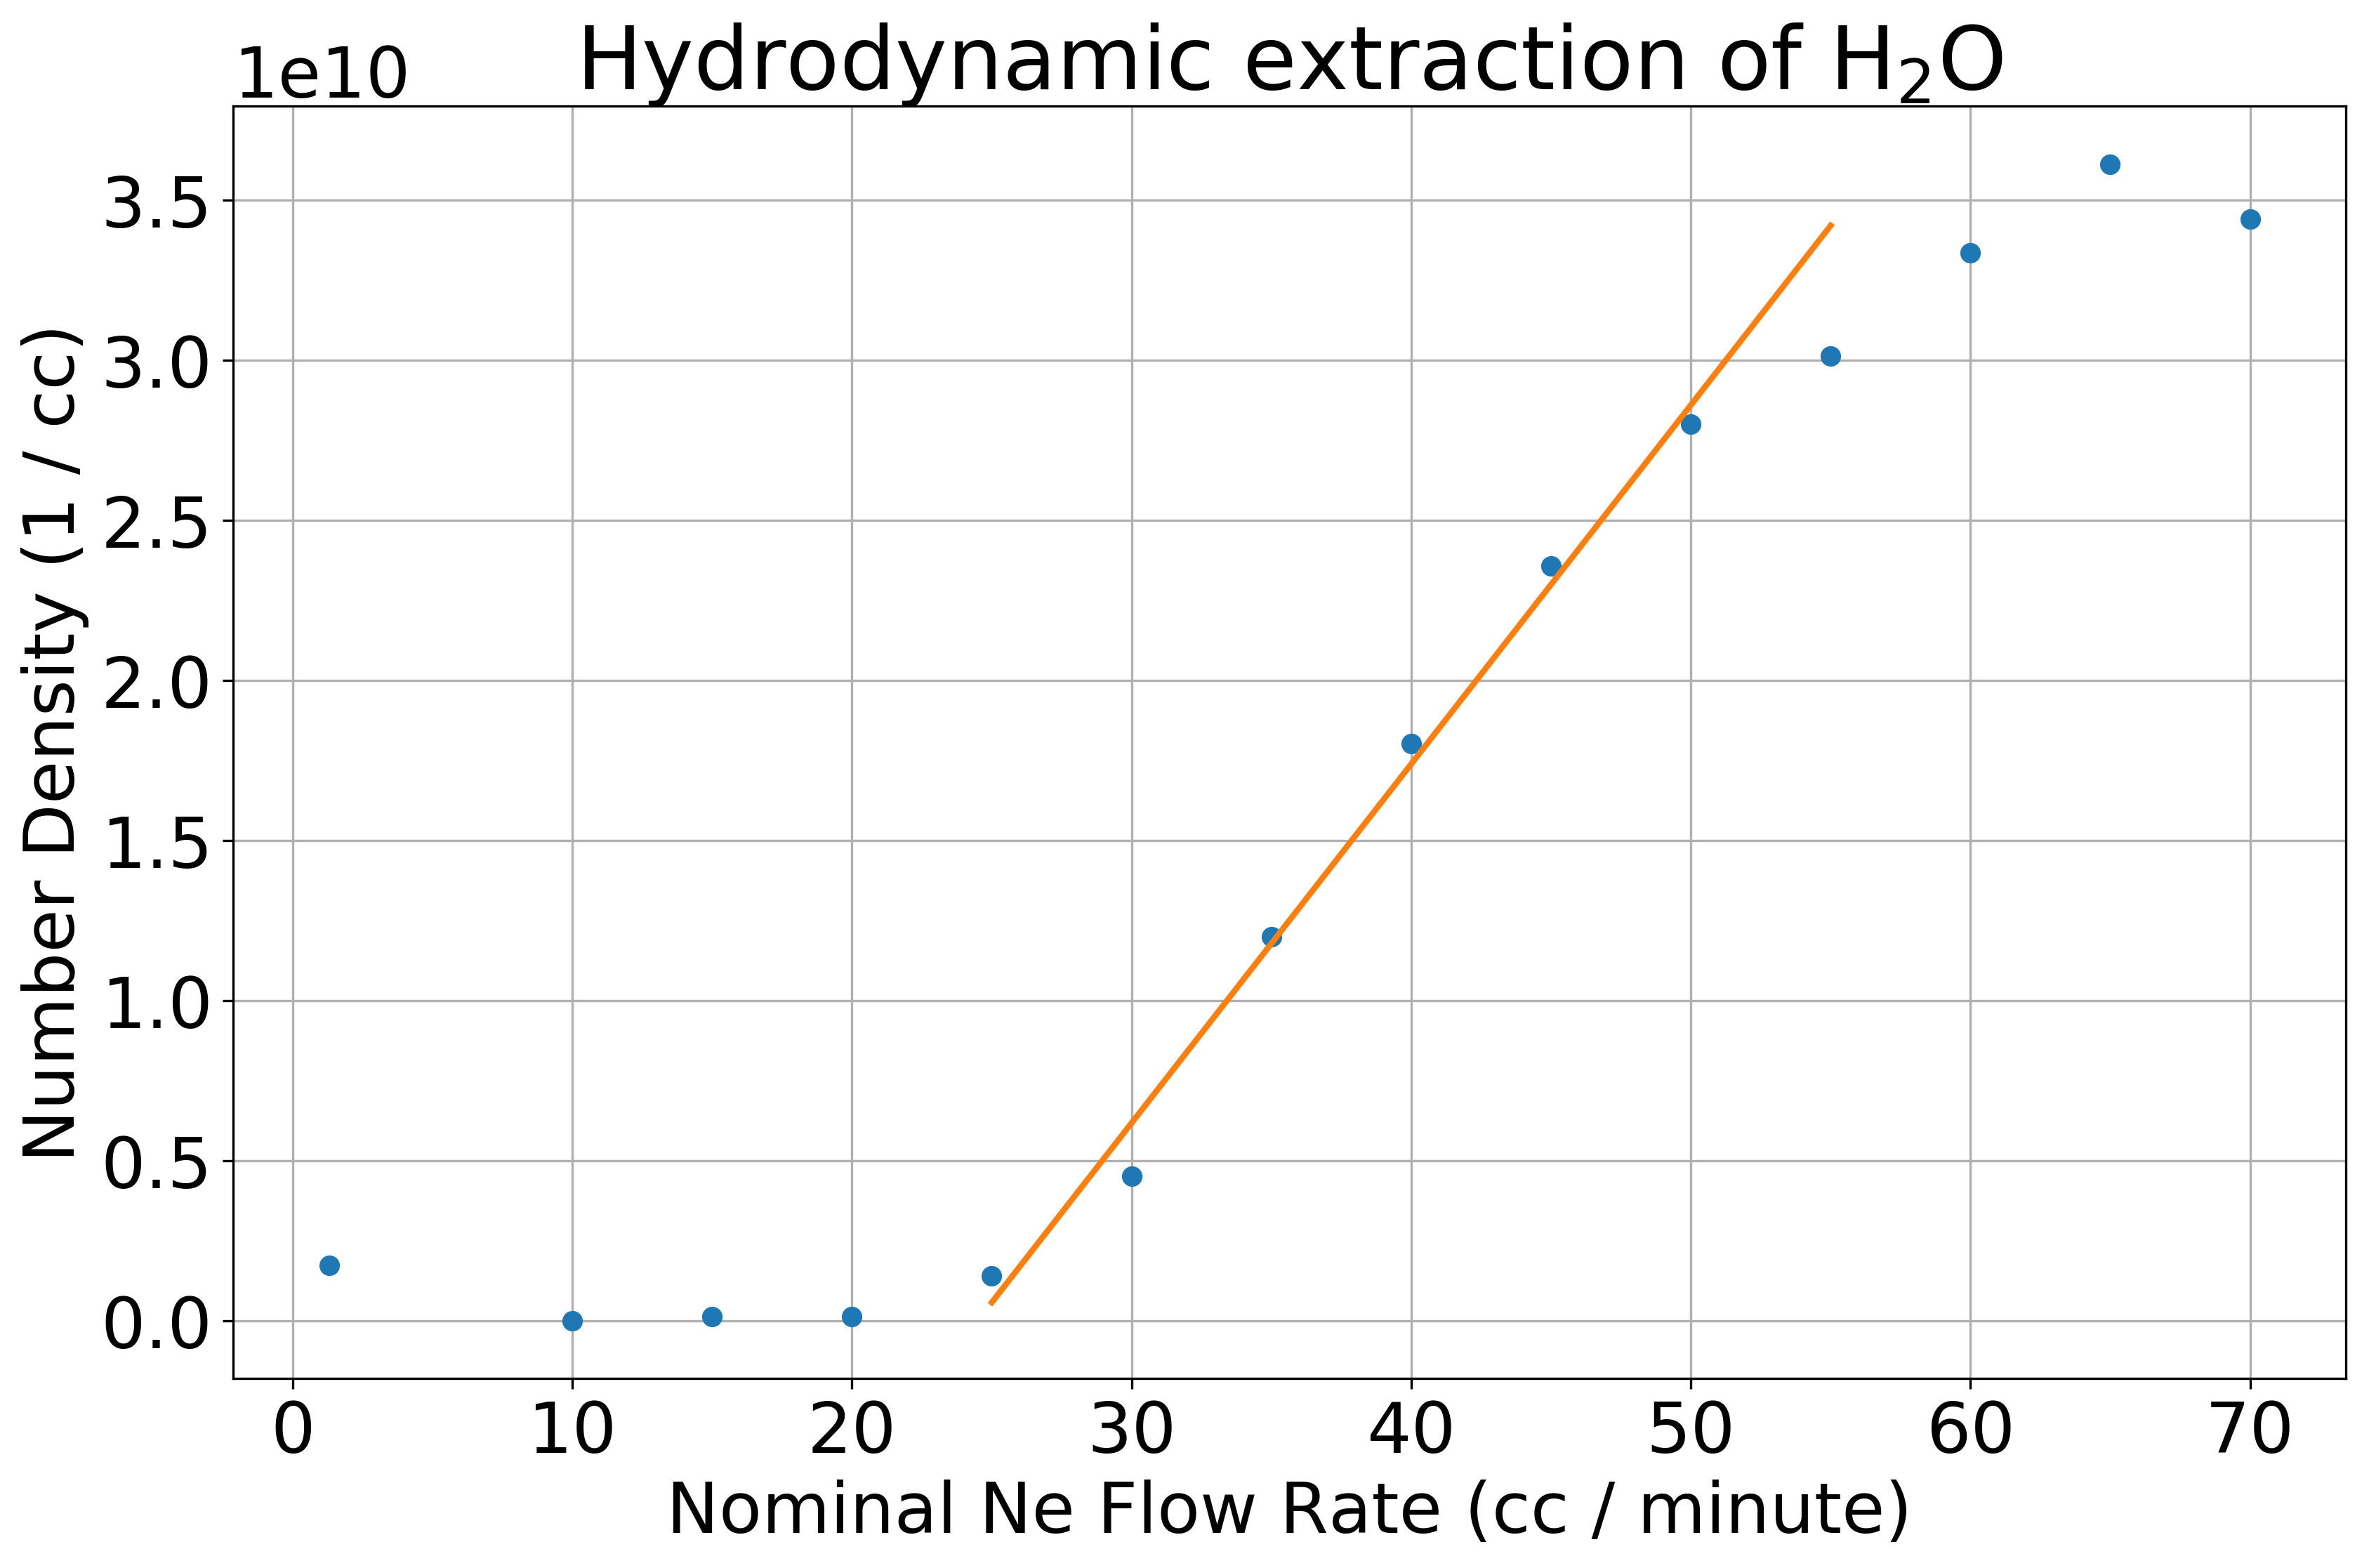
\includegraphics[width=1\textwidth]{CBGB_hydrodynamic_fit.png}
\caption{$1.12 \times 10^9 x + -2.75 \times 10^10$}
\label{f: rga}
\end{figure}

We know have previously calculated the possible number densities of the buffer gas with varying aperture sizes and flow rates. But now we can utilize those equations with the data on the target species to plot out the range of densities that we may see at the trap center as a function of the various apertures that we may utilize.

Knowing from our previous calculations:

$$ \bar{v} = \sqrt{\frac{8 k_B T}{m \pi}} $$
$$ n_{0,b}=\frac{4 f}{A_{aperture} \bar{v}} $$
$$n(z)=\frac{n_o}{2}\left(1-\frac{z}{\sqrt{z^2+a^2}}\right)$$

We can put it all together to get:

$$n(z)=\alpha\frac{f}{A_{aperture} \bar{v}}\left(1-\frac{z}{\sqrt{z^2+a^2}}\right)$$

But what we really care about is the region in which the number density is linearly dependent to the buffer gas flow rate, not over all possible ranges; we've seen that the target species only behaves linearly once it has been entrained in the buffer gas. This means that we should be equating the function of $n(z)$ with the linear fit performed on the data for the parameters the data was taken at.

$$mf+b = \alpha\frac{f}{A_{aperture, o} \bar{v_o}}\left(1-\frac{z_o}{\sqrt{z_o^2+a_o^2}}\right)$$

let

$$\beta = \frac{1}{A_{aperture, o} \bar{v_o}}\left(1-\frac{z_o}{\sqrt{z_o^2+a_o^2}}\right)$$

$$\alpha=\frac{m}{\beta}+\frac{b}{\beta f}$$

Thus, we may get a final form that incorporates the linear slope's dependence on the other variables of the system as well as the overall experimentally derived scaling factor from the data.

$$n(z)=\frac{mf+b}{A_{aperture} \bar{v} \beta}\left(1-\frac{z}{\sqrt{z^2+a^2}}\right)$$

There is a mass dependence in the thermal velocity equation, which leads us to conclude that the choice of the species is a statement of the effecacy of the beam itself. If we choose to calculate the thermal velocity of the target species found in the beam due to the theoretical thermal velocity of the buffer gas, that indicates that the beam properties are still dominated by the buffer gas species. This may not be the case, as we see in our data, we have a ratio of about 10:1, this is pushing the boundaries of the assumption that the buffer gas far outnumbers the target species. At these ratios, we may start to see the effects of the target species on the beam properties.

\begin{figure}[H]
\centering
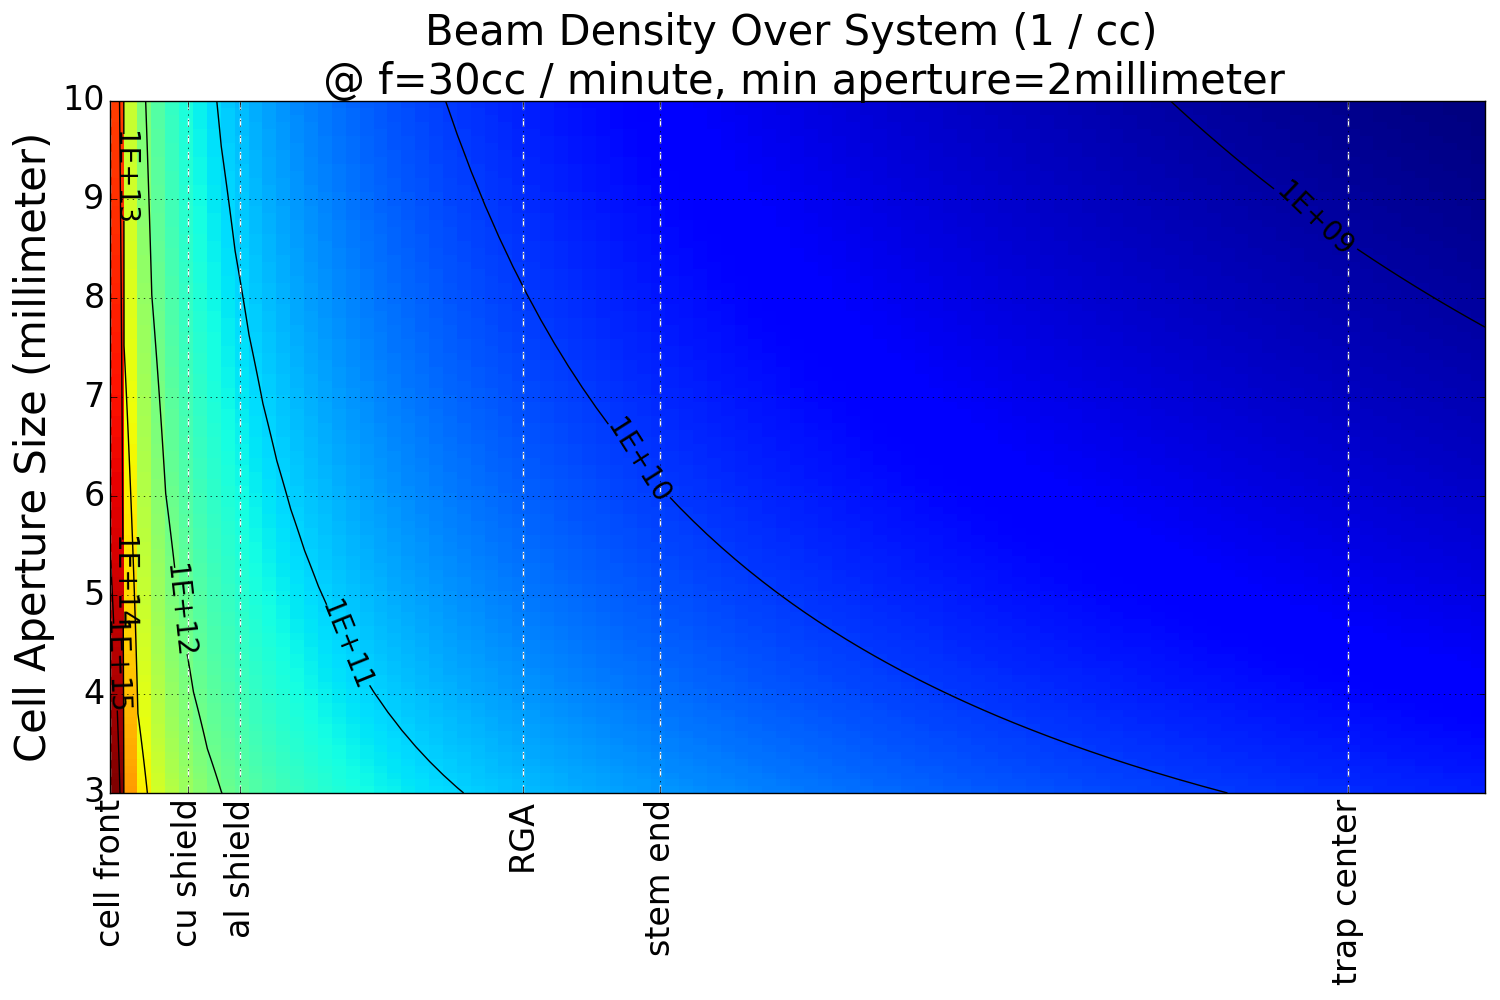
\includegraphics[width=1\textwidth]{CBGB_beam_density_over_system.png}
\caption{}
\label{f: beam_density}
\end{figure}

Extrapolating the fit and estimated density from figure \ref{f: rga}, we can estimate the density of the water at various locations along the beam line as shown in figure \ref{f: beam_density}. We find that we should be able to produce an appreciable number density of water down at the trap center.

From the RGA, we were able to open and close a shutter in the beam path and see an extinction of the water signal, but a more accurate representation would be from the ions in the trap themselves. We know that the trapped $Be^+$ ions will reaction with $H_2O$ to predominately produce $BeOH$, which we see as a drop in the fluorescence. Figure \ref{f: shutter_closing} shows fits of the fluorescence decay as a beam from the CBGB is suddenly blocked by our shutter in the beam line. Comparing the fitted reaction rates, we find that they agree with the background rates found as shown in figure \ref{f: shutter_bkg}. This indicates to us that we indeed have a beam of cryogenic water coming from the CBGB, as seen by the sudden extinction of the $Be^+ + H_2O$ reaction.

\begin{figure}[H] \label{f: shutter_bkg}
\centering
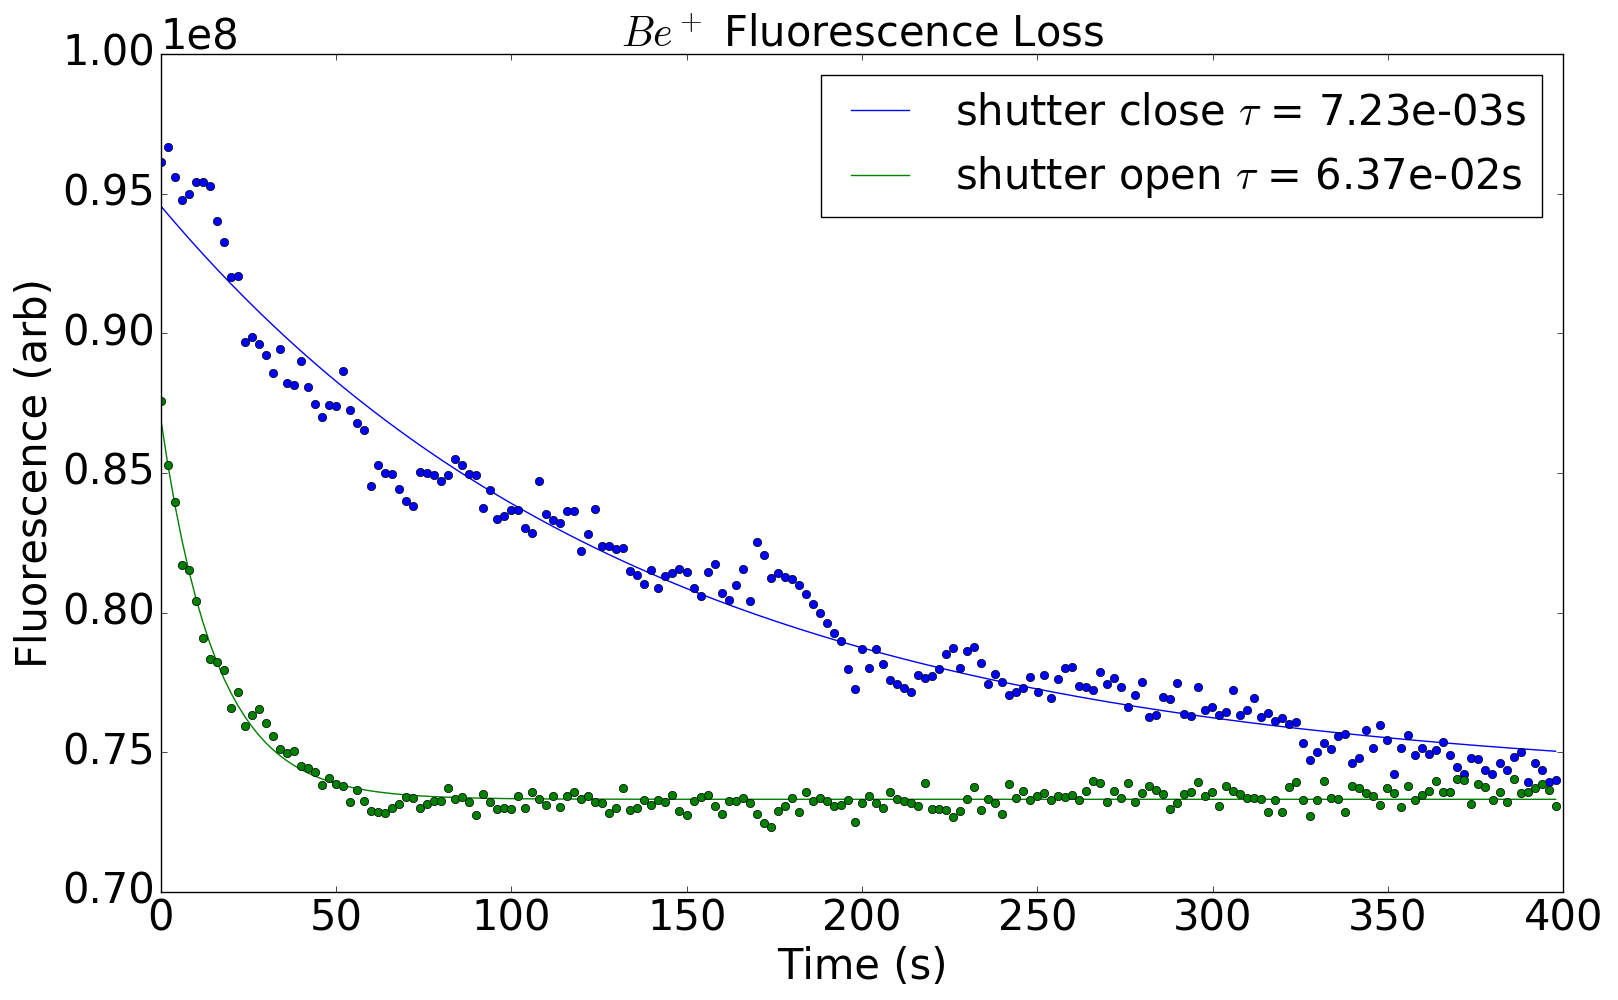
\includegraphics[width=1\textwidth]{CBGB_sudden_shutter_flow_bkg.png}
\caption{}
\end{figure}

\begin{figure}[H] \label{f: shutter_closing}
\centering
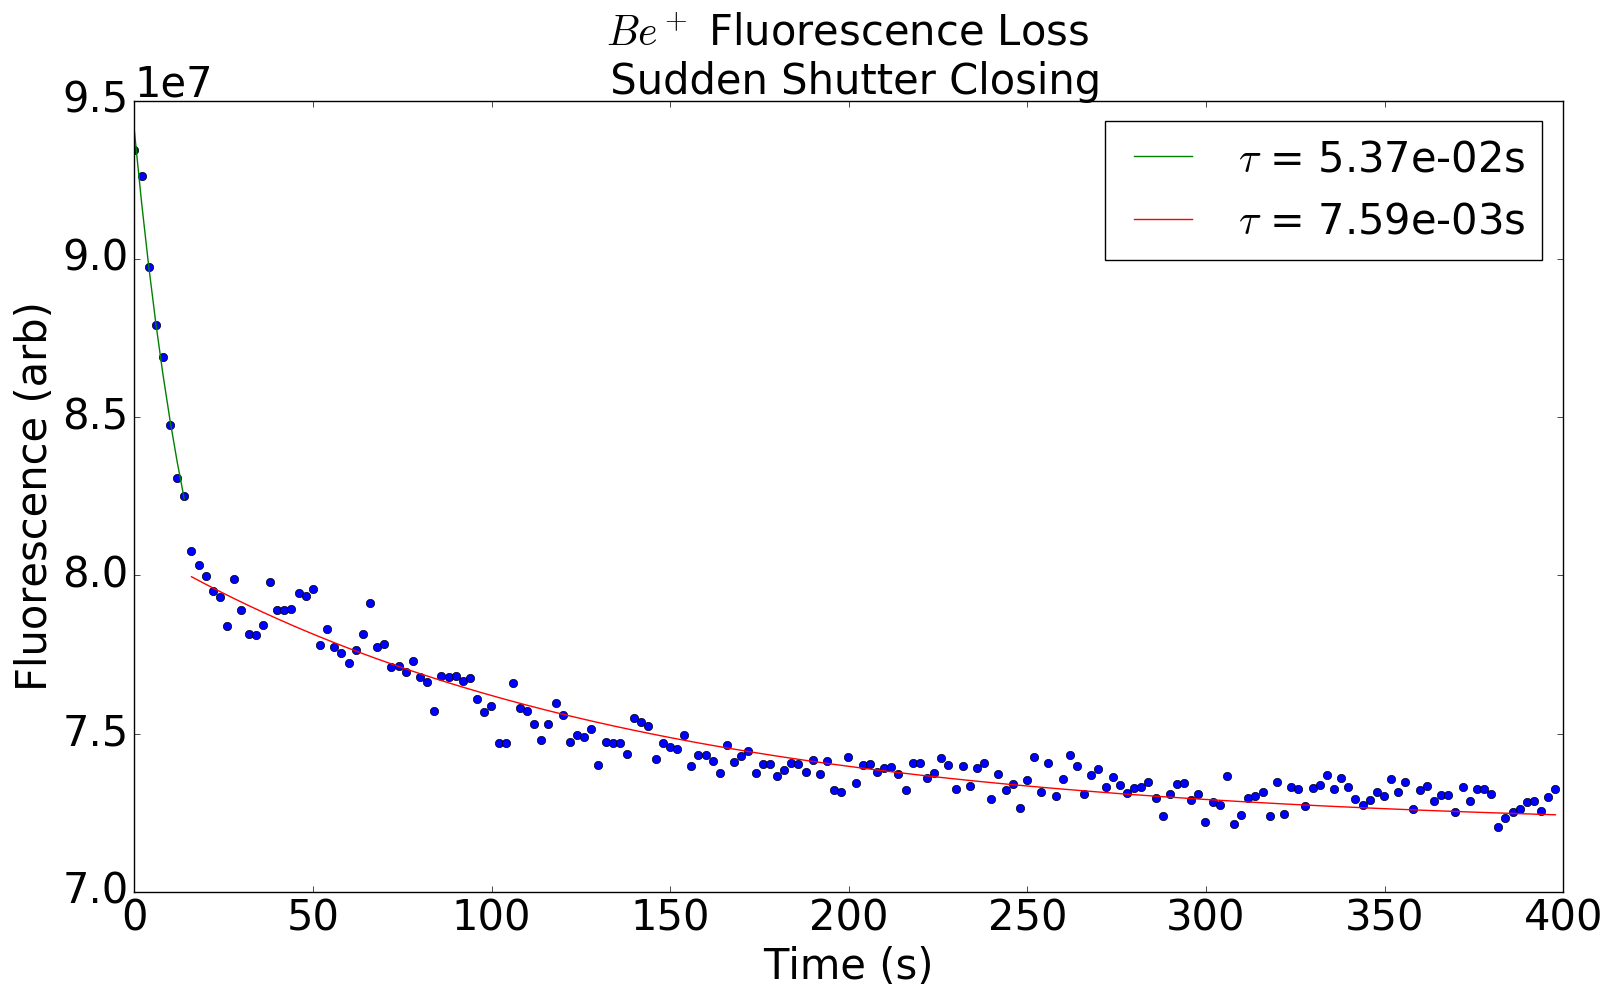
\includegraphics[width=1\textwidth]{CBGB_sudden_shutter_flow.png}
\caption{}
\end{figure}

\subsubsection{Beam Velocity}

To better understand the reaction temperatures we will be able to reach, we need a characterization of the beam's velocity, more specifically, the velocity of the target species entrained within the buffer gas. By ablating ytterbium into the neon buffer gas, we find that the ytterbium is entrained within the neon and sympathetically cooled to the cell's temperature. As long as the target species number density is a trace amount in comparison to the bulk buffer gas number density (1:1000), the flow characteristics are dominated by the buffer gas species \cite{Hutzler2012}. The forward velocity of the beam is not only parameterized by the temperature of the buffer gas species, it is also dependent on the flow regime. As we increase the flow of neon into the cell, figure \ref{f: rga} shows a linear increase in the $H_2O$ signal from a downstream RGA. This coincides with the beam operating within the intermediate flow regime, where there are few collisions at the cell aperture, resulting in a slight forward boosting and increased extraction efficiency of the target species. At higher flow regimes, entering the supersonic regime, we would see a "freeze out" where the forward velocity reaches $1.4\bar{v}$ and we would not see appreciable gains in species extraction \cite{Hutzler2012}. We chose to operate at a nominal neon flow rate of 30 sccm based upon the reaction rate of the ions downstream.

\begin{figure}[H]
\centering
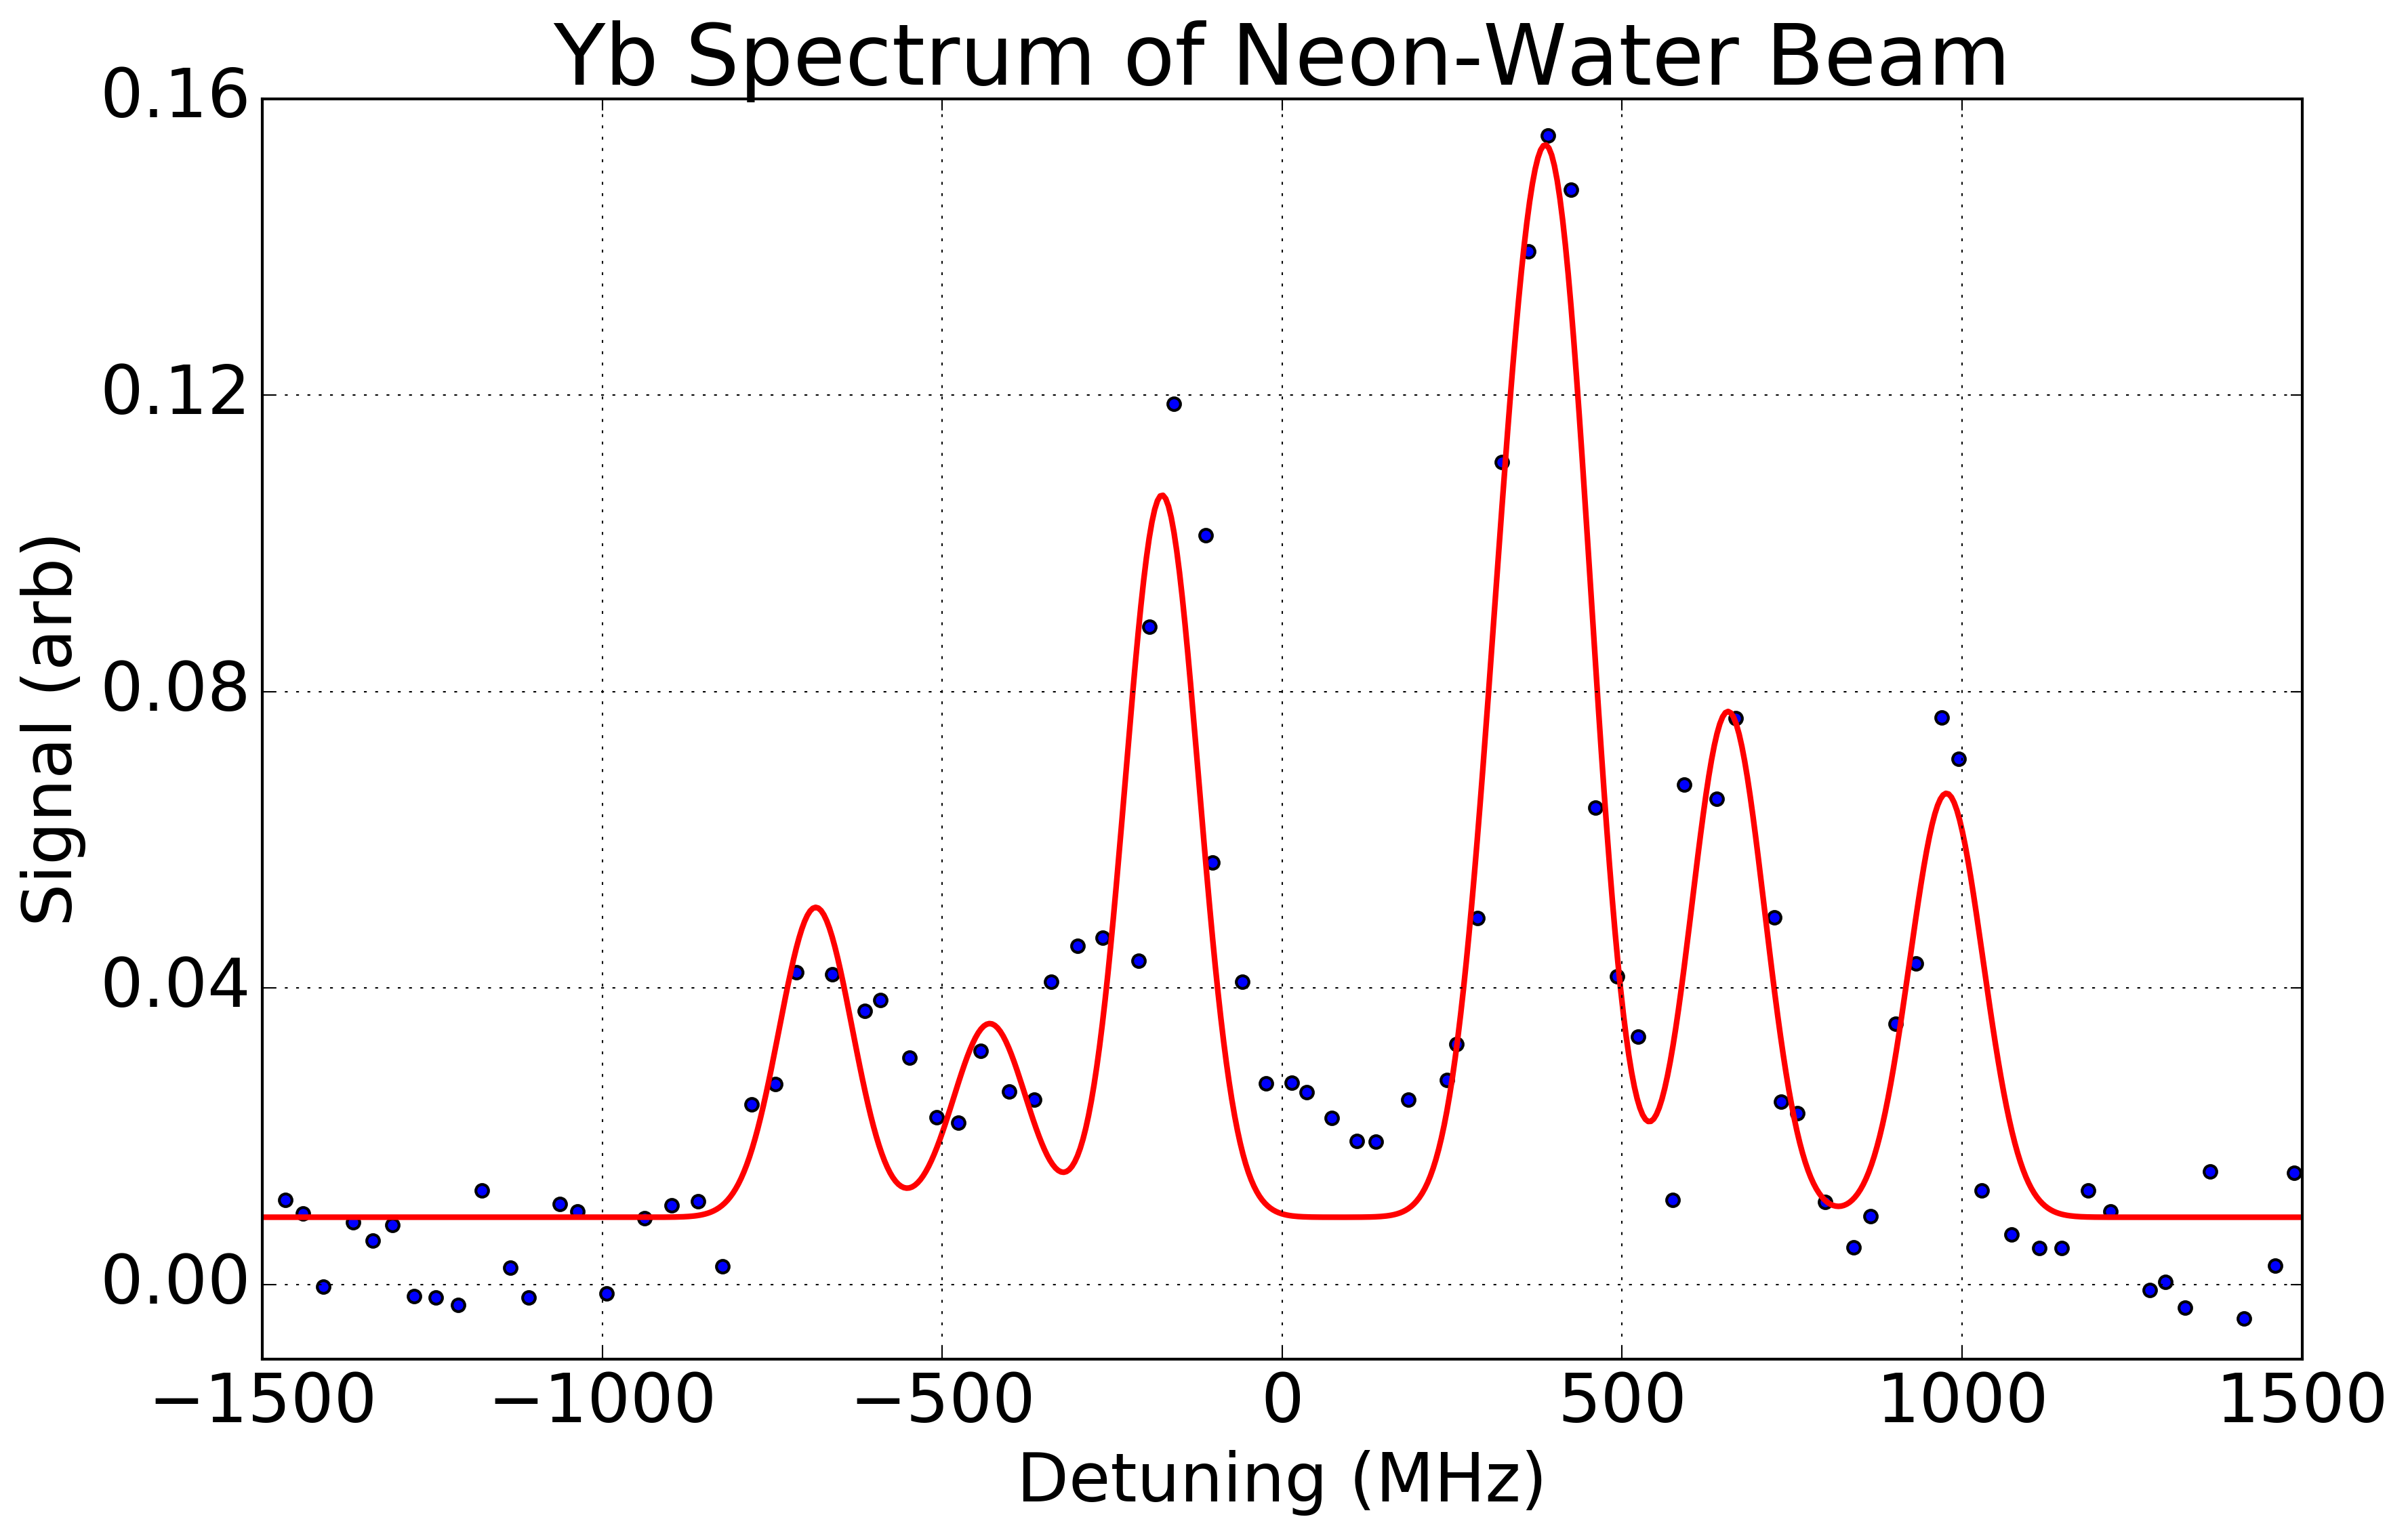
\includegraphics[width=1\textwidth]{CBGB_yb_spectrum_long.png}
\caption{\label{f: yb_spectrum}}
\end{figure}

\subsection{Be$^+$ + H$_2$O}

In loading both Be$^+$ and C$^+$ in the trap and exposing them to H$_2$O from the leak valve, we find that the two proceed at drastically different rates, which does not make sense looking at capture rates. We investigate the rate of Be$^+$ + H$_2$O since C$^+$ + H$_2$O proceeds at the capture limit.

\section{Be$^+$ + O$_2$}
Beryllium metal is ablated with an Nd:YAG laser and trapped in a linear Paul trap. Laser cooling is applied with a 313nm laser. Pure O$_2$ gas is introduced into the chamber via leak valve to react with the ions. Remaining reactants and charged reaction products are ejected into a time-of-flight mass spectrometer (TOF) where the various masses of ions can be determined.

When the Be$^+$ is excited from the $^2$S$_{1/2}$ to the $^2$P$_{3/2}$ manifold, we find the energetically allowed channels to be:

\begin{align}
    \text{Be}^+(^2\text{P}_{3/2}) + \text{O}_2 & \to \text{O}_2^+ + \text{Be} \label{eq: o2+} \\
    & \to \text{BeO}^+ + \text{O}_2 \label{eq: beo+} \\
    \text{Be}^+(^2\text{P}_{3/2}) + \text{H$_2$O} & \to \text{BeOH}^+ + \text{H} \\
    \text{Be}^+(^2\text{P}_{3/2}) + \text{H}_2 & \to \text{BeH}^+ + \text{H} \\
    \text{BeH}^+ + \text{H$_2$O} & \to \text{BeOH}^+ + \text{OH}
\end{align}

Without excitation into the $^2$P$_{3/2}$ manifold, reactions \ref{eq: o2+} and \ref{eq: beo+} are endothermic by 2.75eV and 1.1eV, respectively. 

Despite the fact that reaction \ref{eq: beo+} is energetically allowed, it is never seen with laser cooling.

Without 313nm light, the Be$^+$ ions stay in the $^2$S$_{1/2}$ ground state, but with a ion trap depth > 4eV, there are portions of the ion cloud with enough energy to still proceed with the production of BeO$^+$. Without the laser cooling, we observe the disappearance of BeO$^+$ from the trap due to exciting the molecule into a pre-dissociative state.

\begin{figure}[H]
\centering
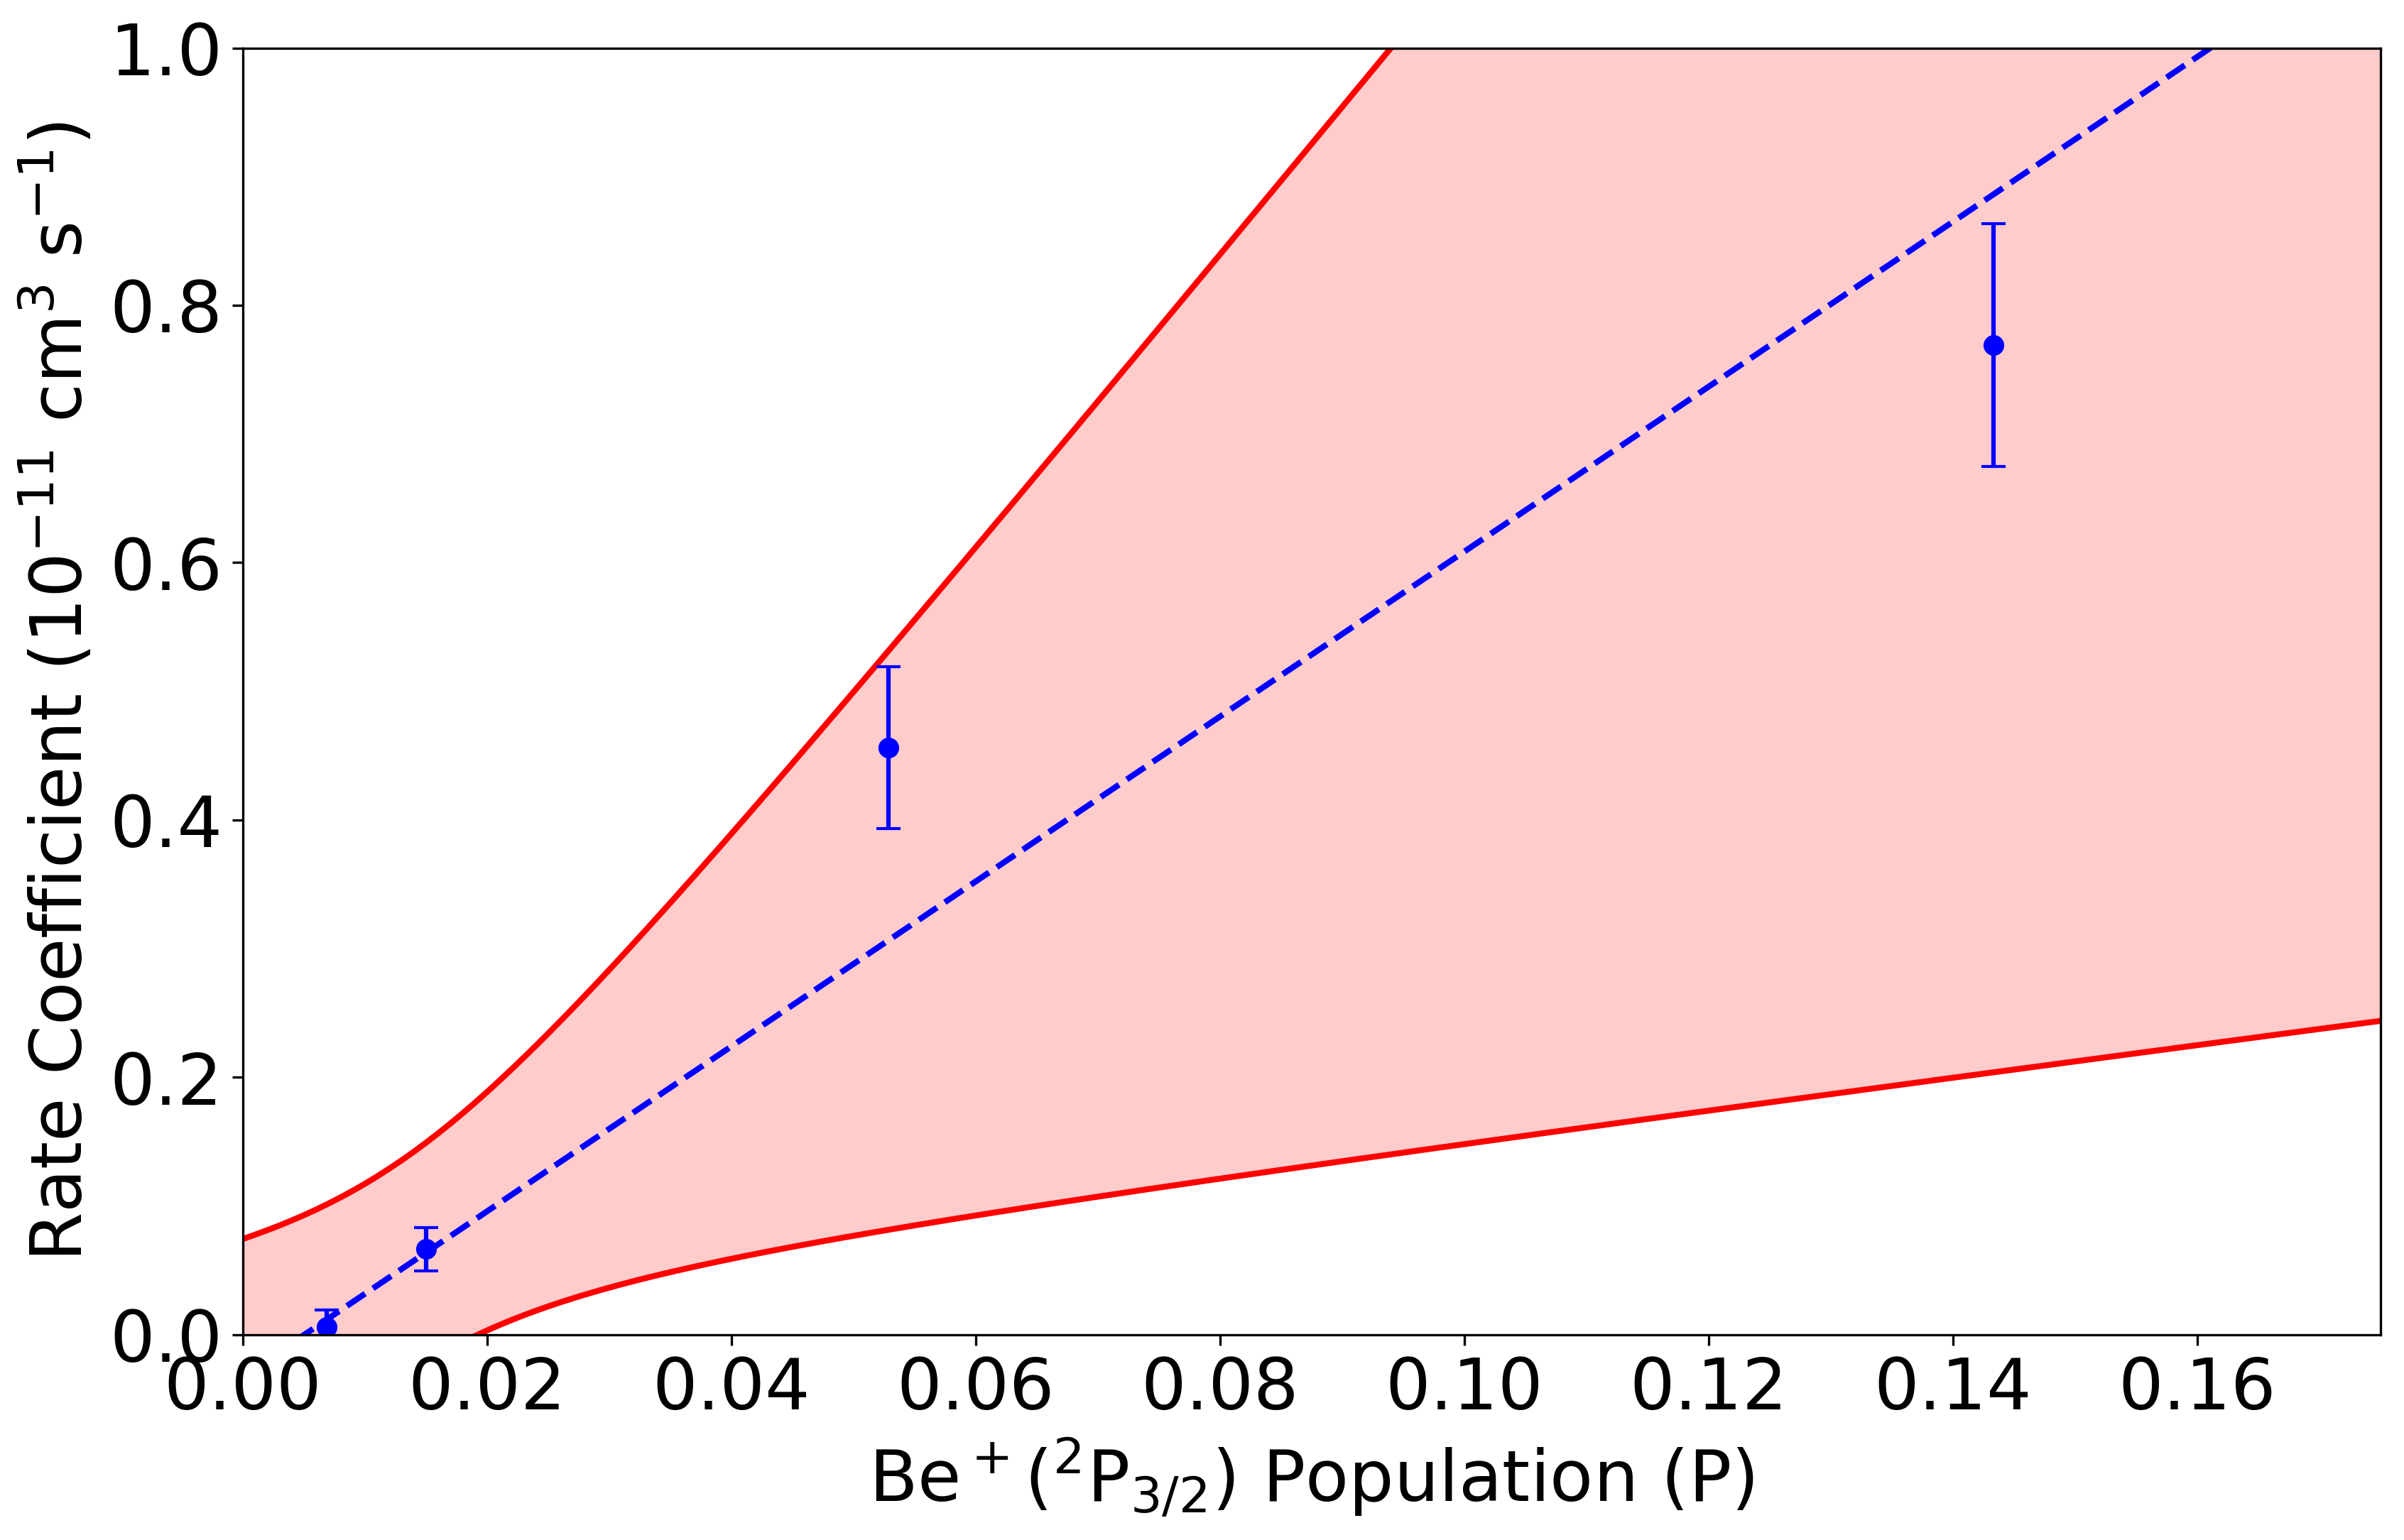
\includegraphics[width=0.7\textwidth]{beo_p_state.png}
\caption{\label{fig: p-state} A linear dependence on the rate constant for reaction \ref{eq: o2+} as a function of P state excitation. $k = (6 \pm 1) \times 10^{-11} P + (-0.03 \pm 0.16) \times 10^{-11}$}
\end{figure}

% \begin{figure}[H]
% \centering
% \includegraphics[width=0.5\textwidth]{p_state_no_b.png}
% \caption{\label{fig: p-state} A linear dependence on the rate constant for reaction \ref{eq: o2+} as a function of P state excitation. Fit $(5.45 \pm 1.03) \times 10^{-11} P$}
% \end{figure}

\begin{figure}[H]
\centering
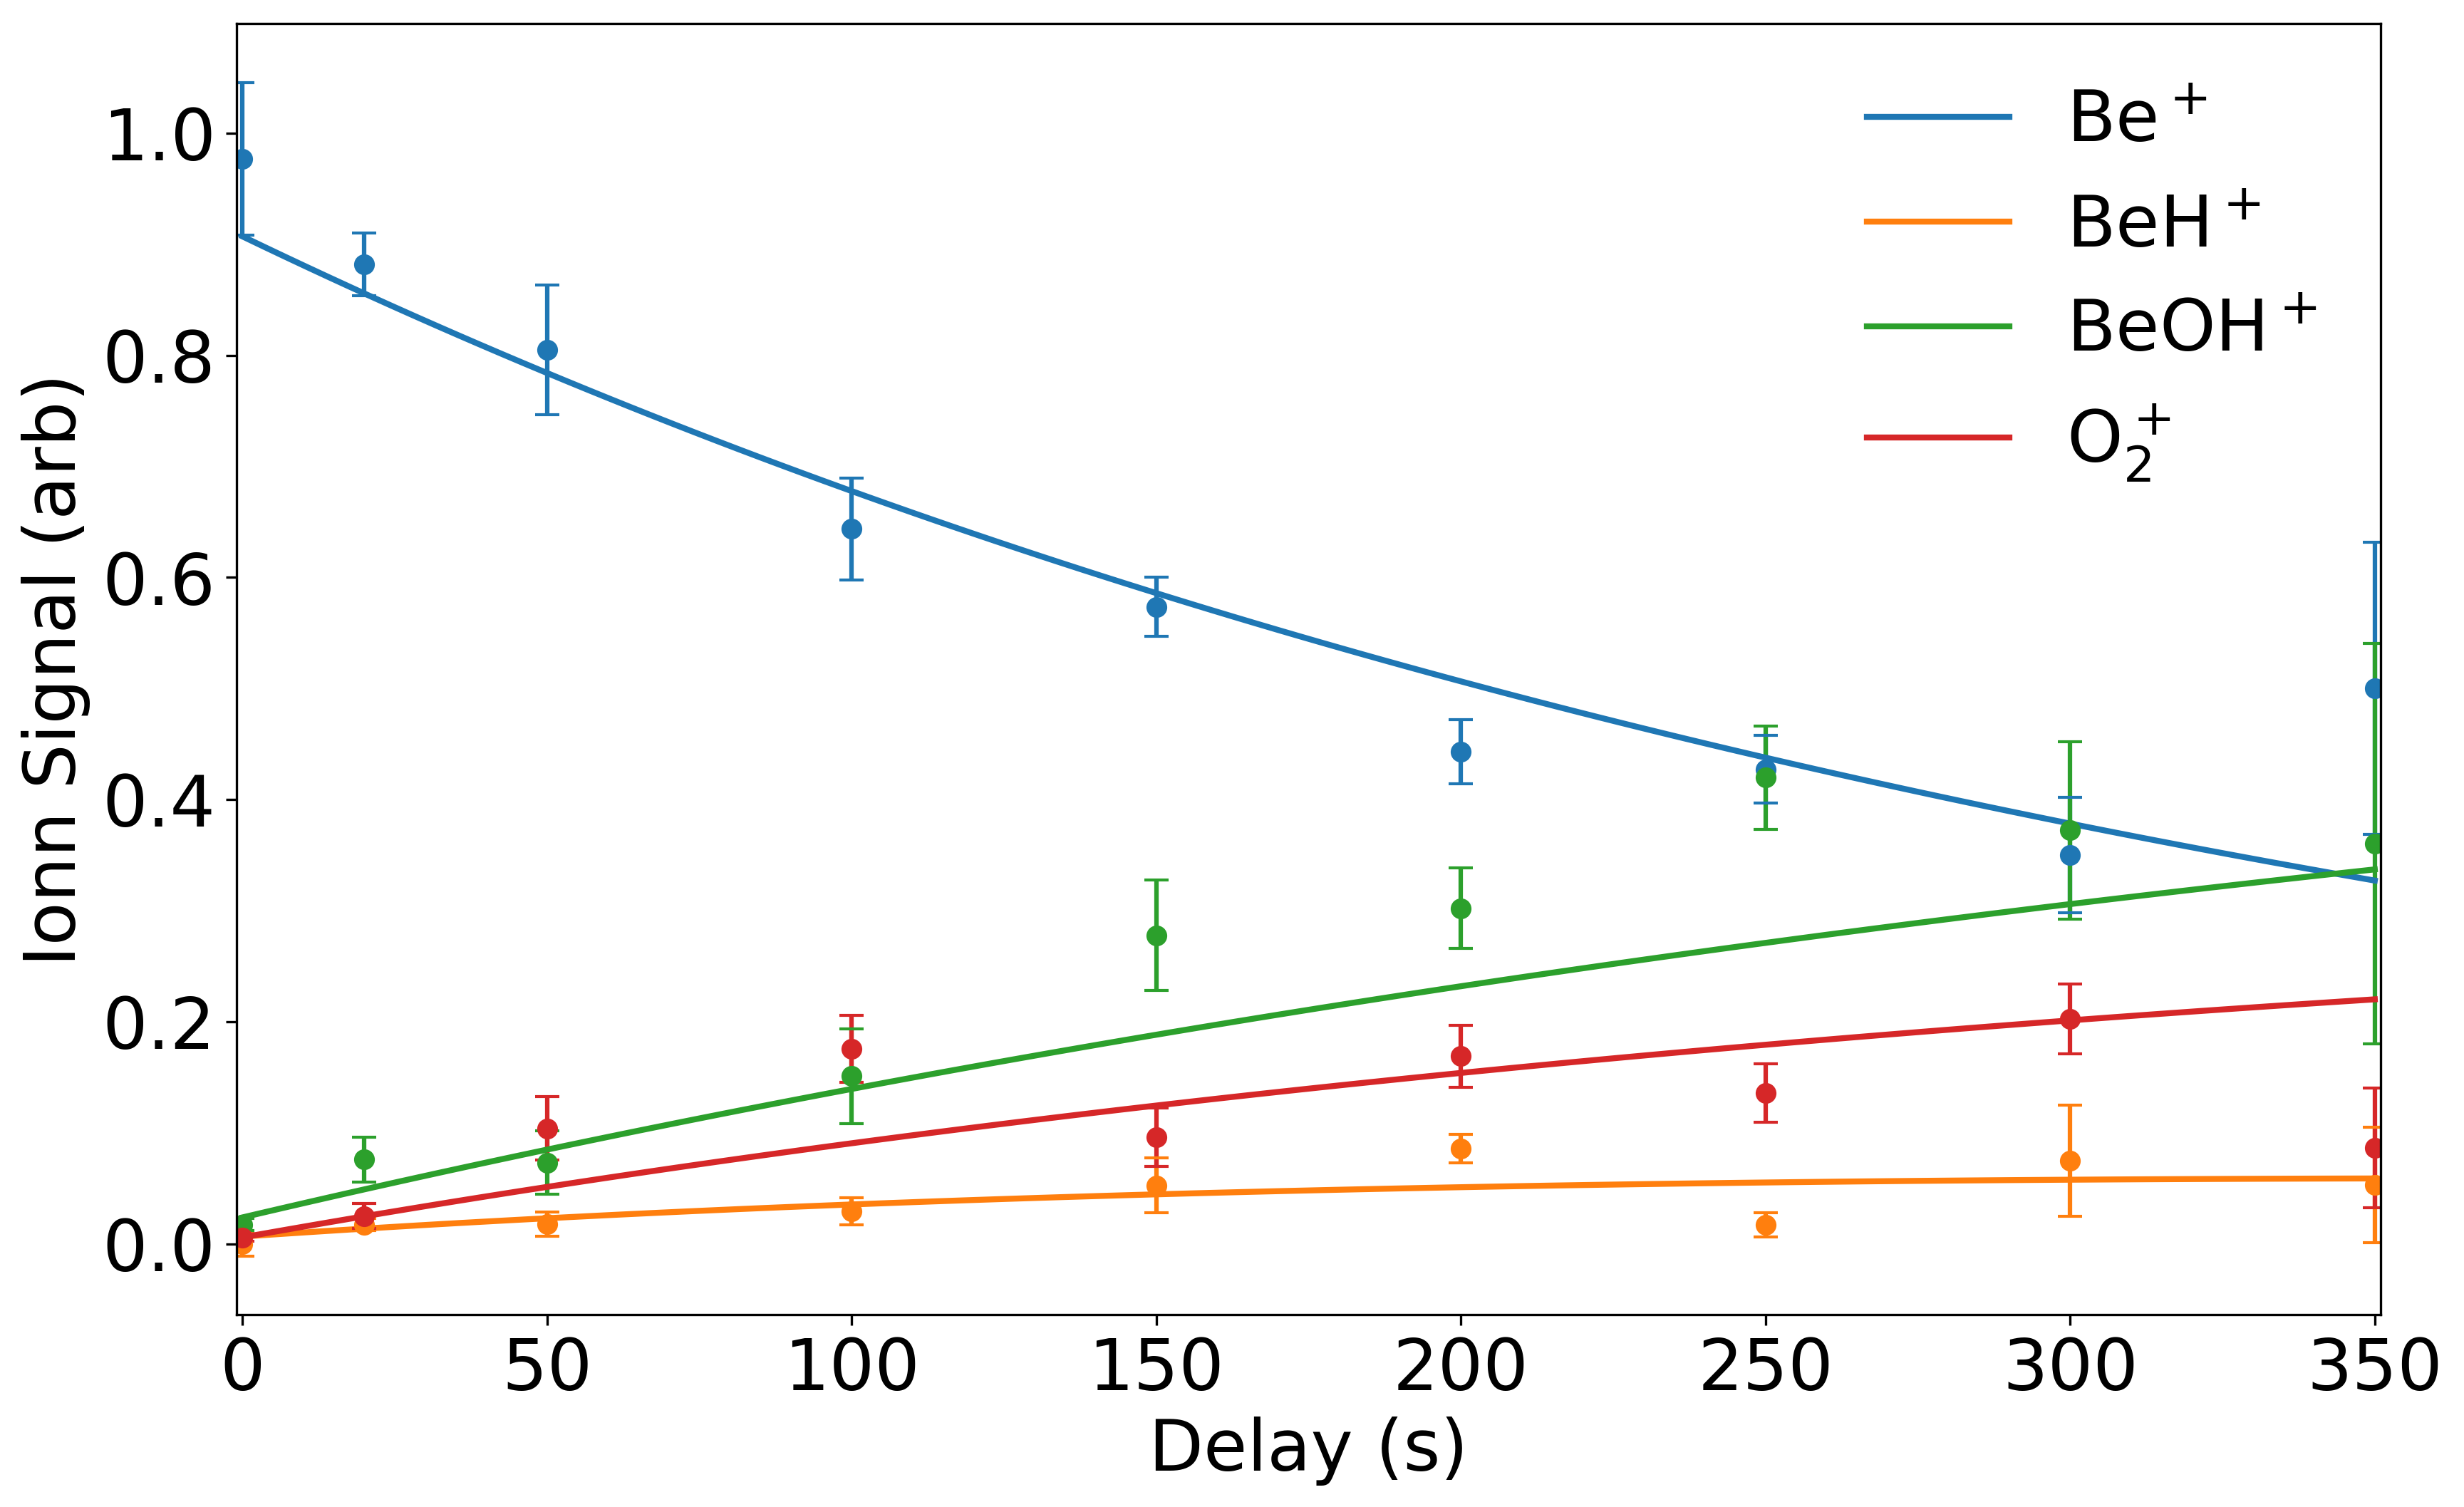
\includegraphics[width=0.7\textwidth]{beo_laser_fit.png}
\caption{\label{fig: laser fit} Shared fitting of trapped products with 14\% p-state excitation.}
\end{figure}

\begin{figure}[H]
\centering
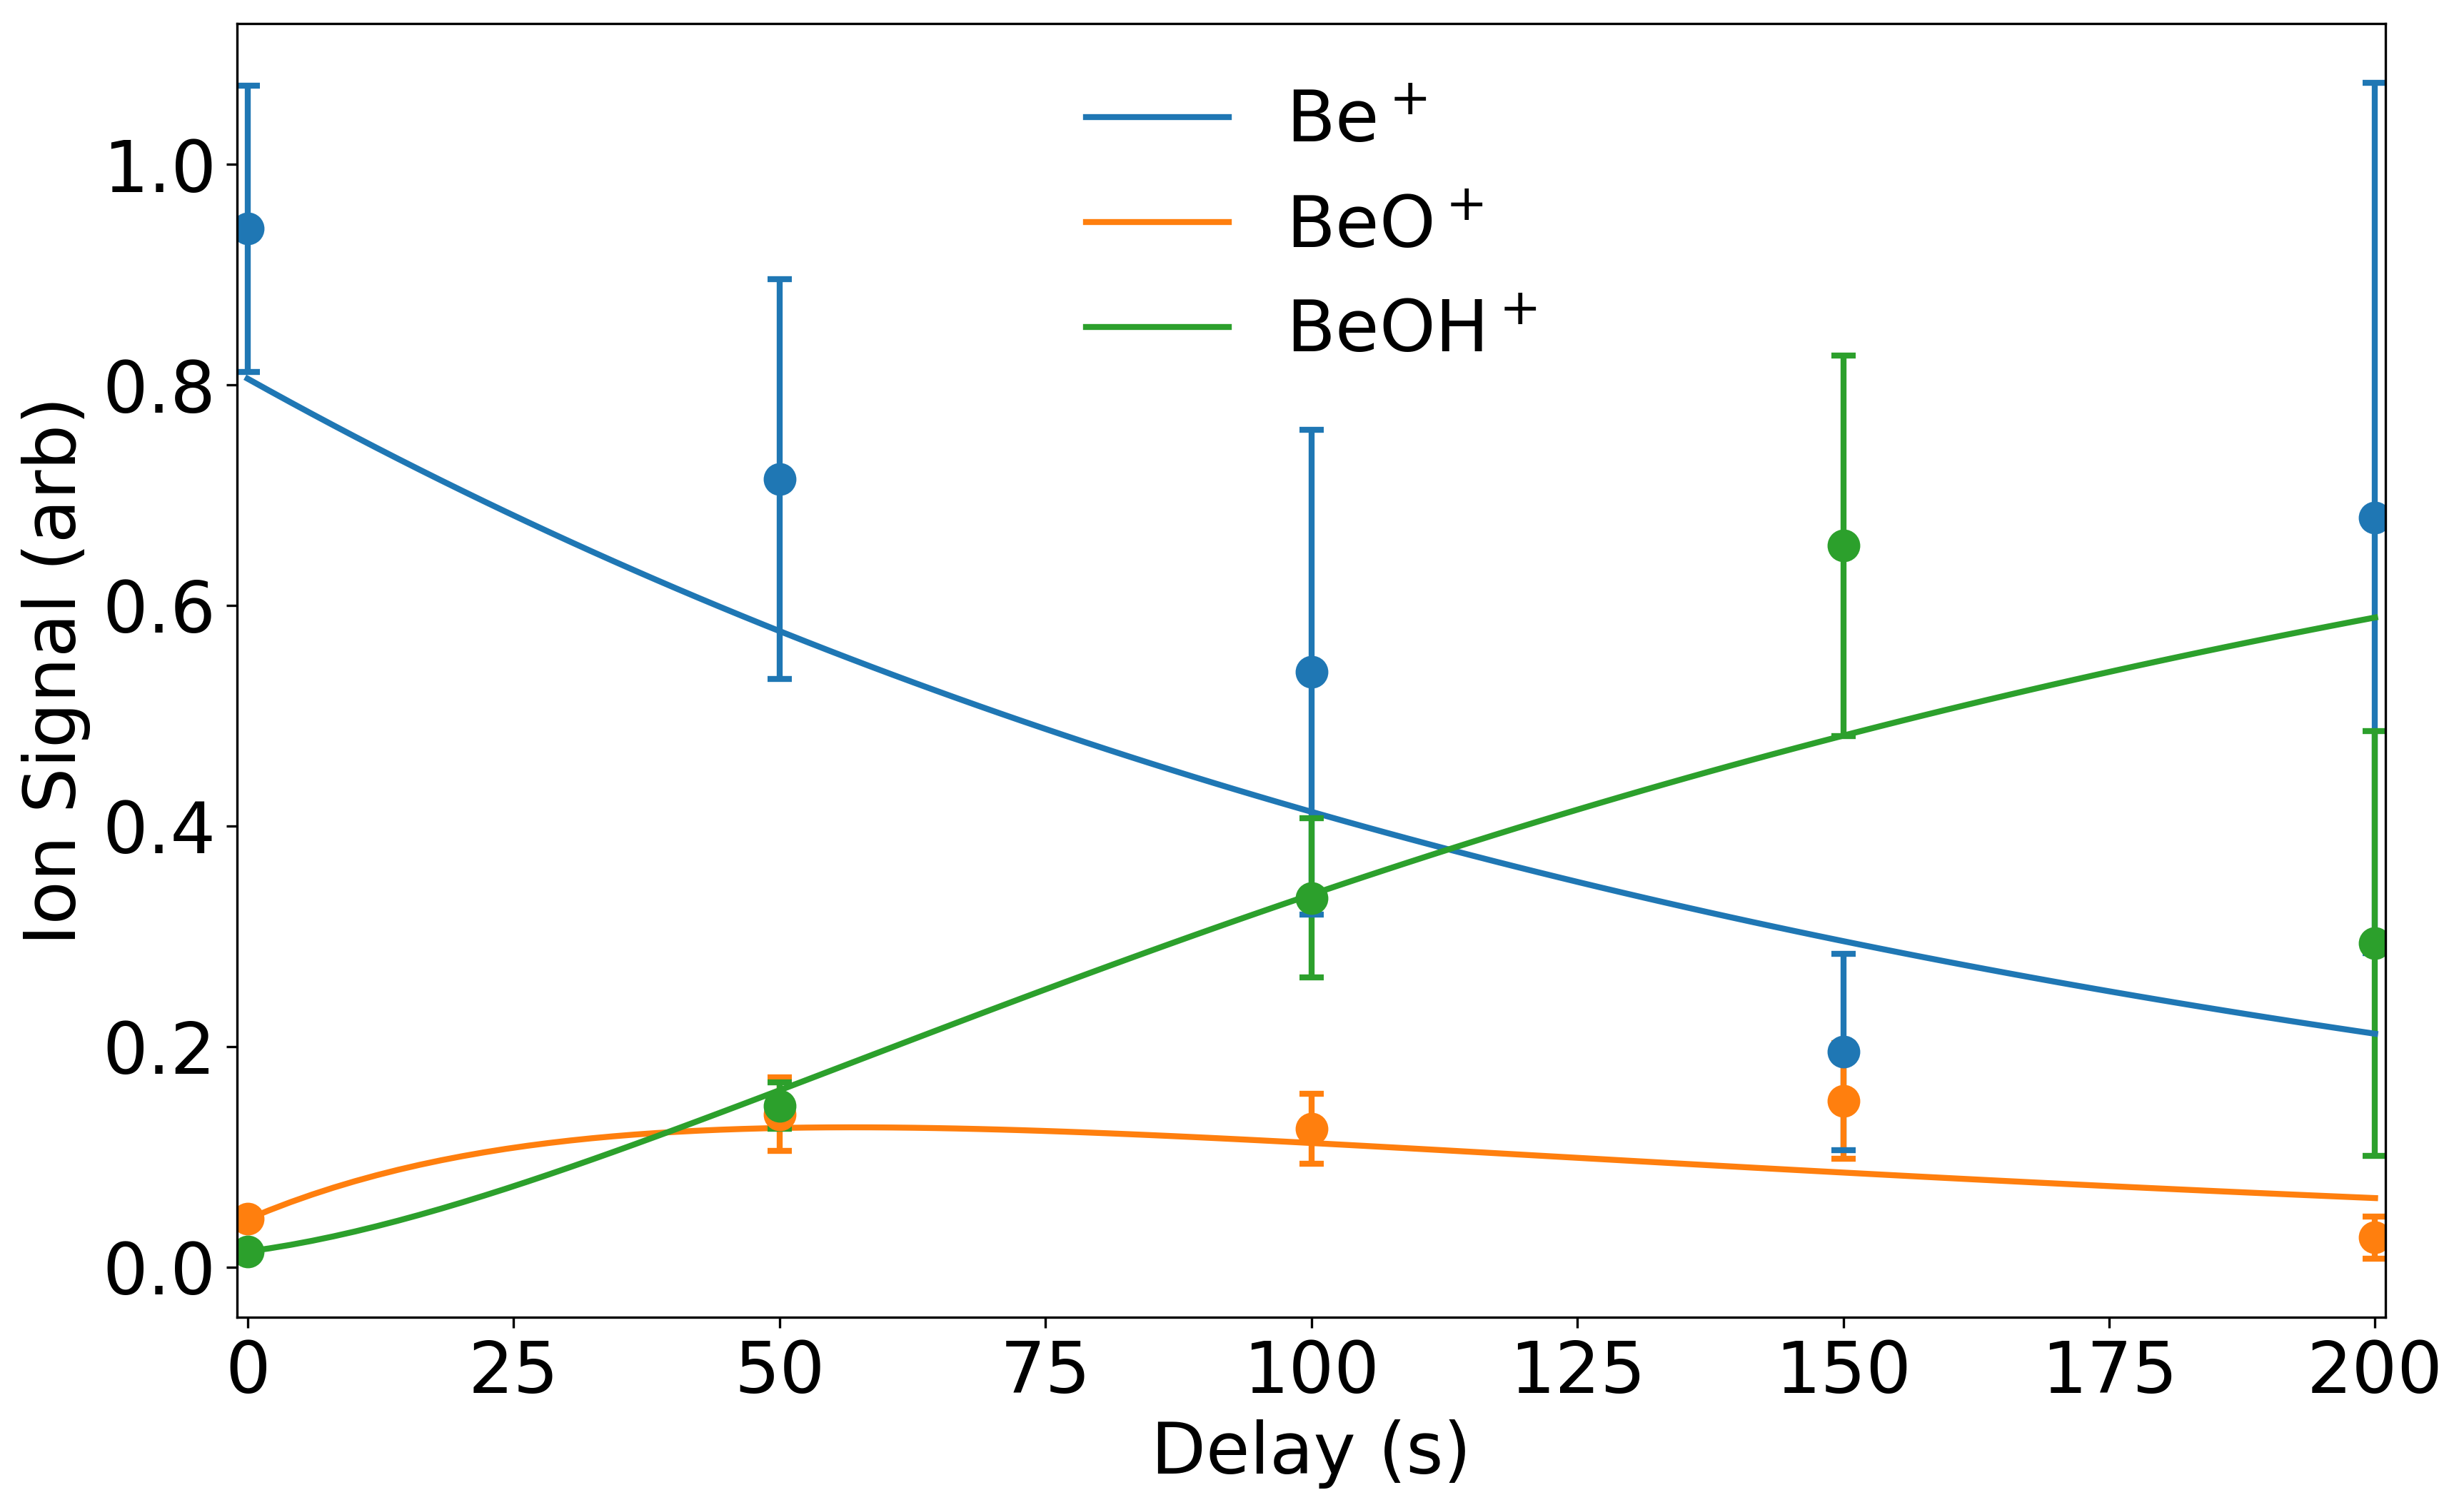
\includegraphics[width=0.7\textwidth]{beo_no_laser_fit.png}
\caption{\label{fig: no laser fit} Shared fitting of trapped products with 14\% p-state excitation.}
\end{figure}

\begin{figure}[H]
\centering
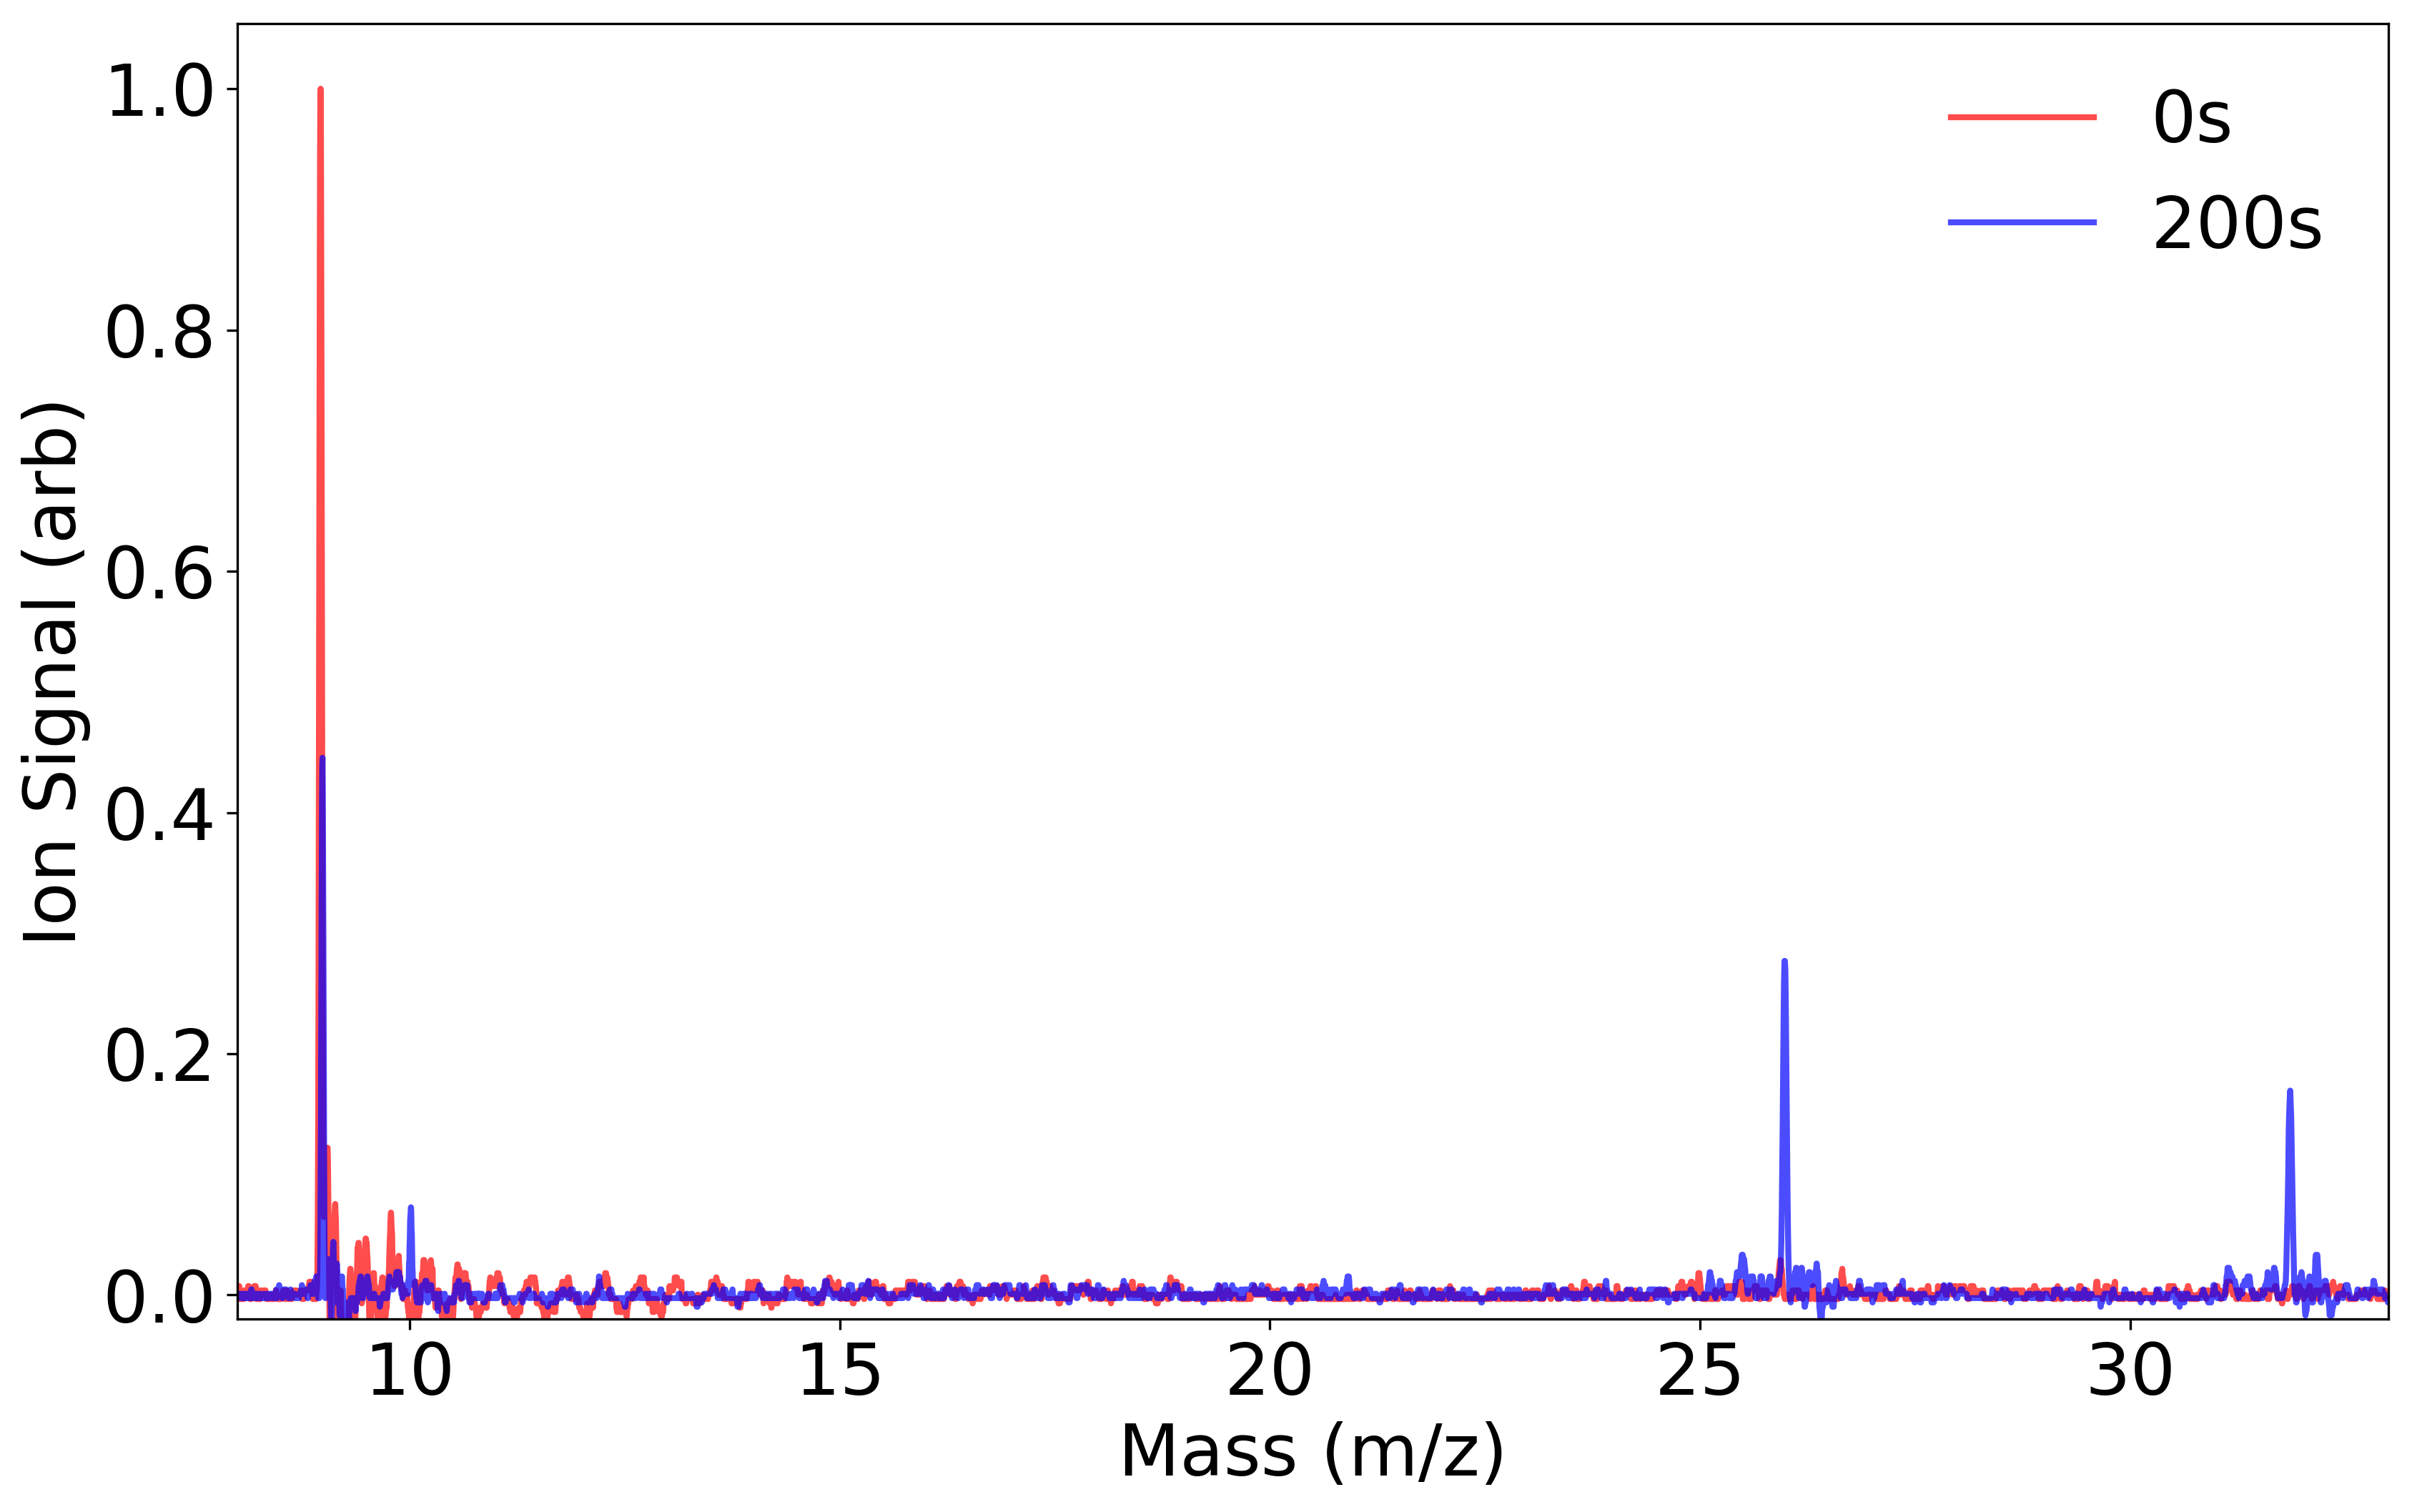
\includegraphics[width=0.7\textwidth]{beo_laser_TOF.png}
\caption{\label{fig: laser TOF} TOF traces for data taken with 14\% p-state excitation at 0s and 200s showing no products at 0s, but distinct peaks for reaction products BeH$^+$, BeOH$^+$, and O$_2^+$.}
\end{figure}

\begin{figure}[H]
\centering
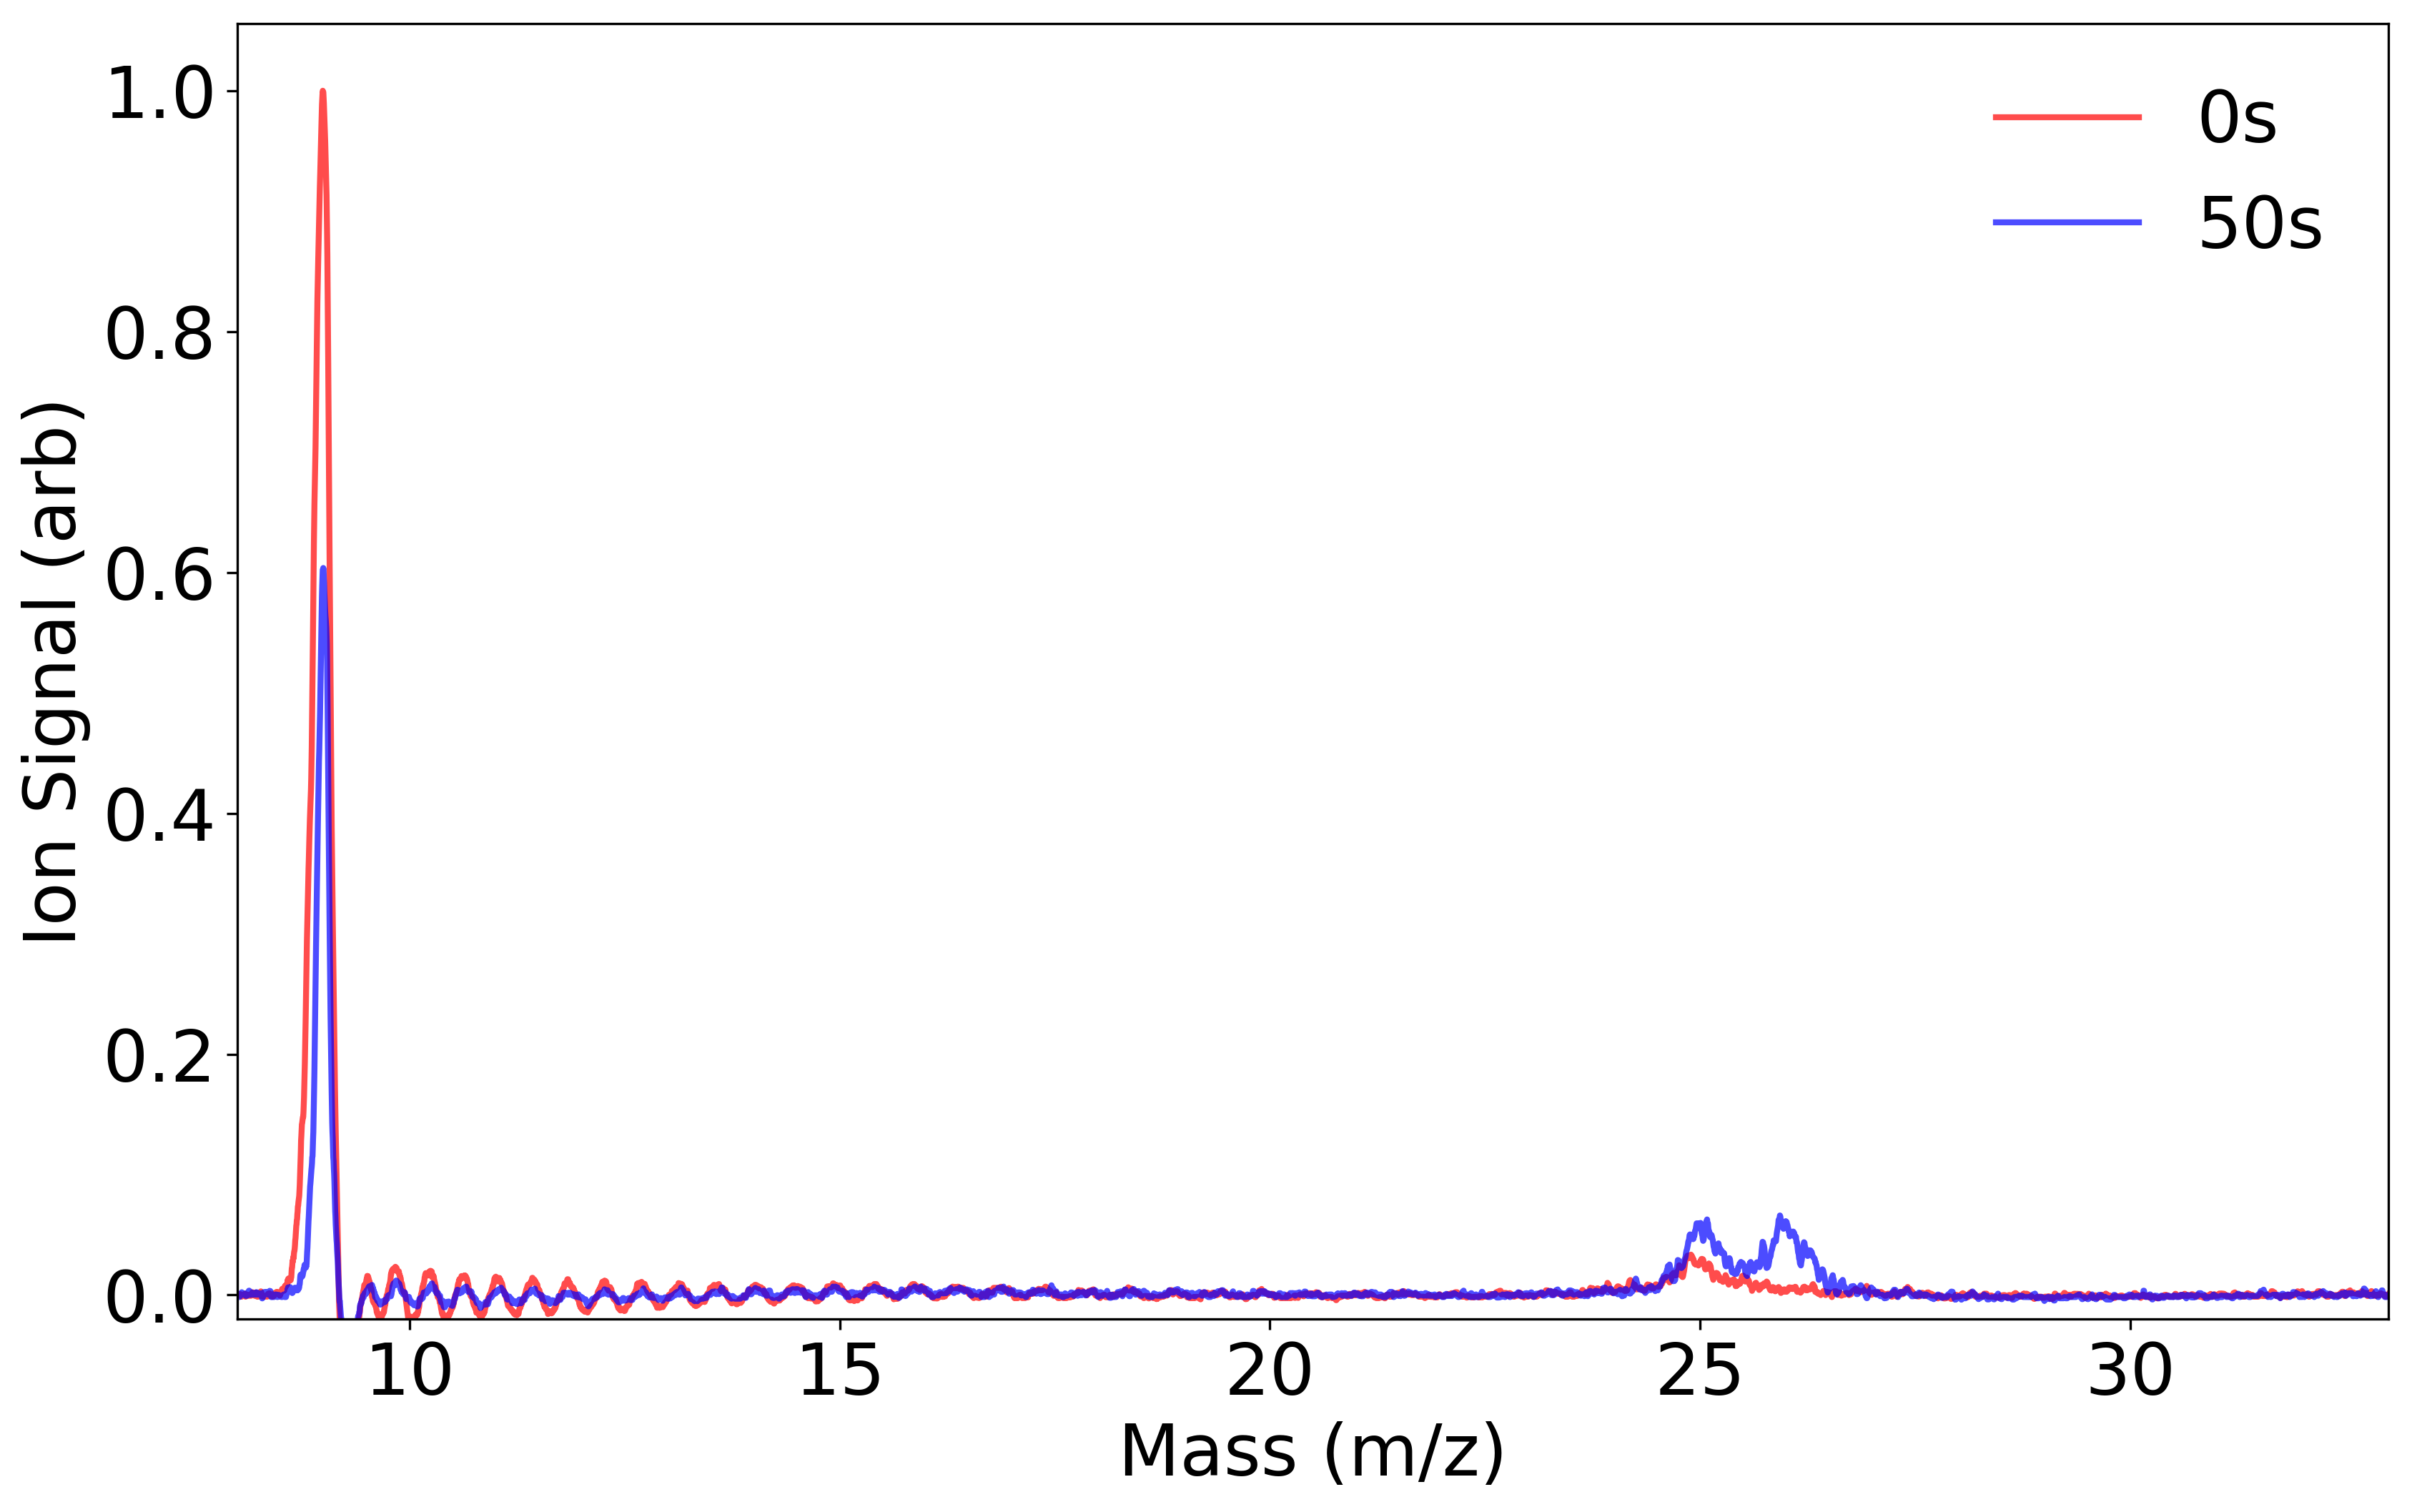
\includegraphics[width=0.7\textwidth]{beo_no_laser_TOF.png}
\caption{\label{fig: non laser TOF} TOF traces for data taken with 14\% p-state excitation at 0s and 200s showing no products at 0s, but distinct peaks for reaction products BeH$^+$, BeOH$^+$, and O$_2^+$.}
\end{figure}

\subsection{State Counting}

\begin{align}
E_{int} & = \omega_e\left(v + \frac{1}{2}\right) - \omega_ex_e\left(v+\frac{1}{2}\right)^2 + B_ej(j+1)
\end{align}

Where $\omega_e$ is the vibrational constant, $\omega_ex_e$ is the anharmonic vibrational constant, $B_e$ is the rotational constant, and $v$, $j$ are vibrational and rotational quantum numbers respectively. You can count how many states there are up to a maximum energy input and compare states to see which product channel is preferred statistically.

To get a more accurate counting, we should be comparing the integrated states including the energy taken away by the other reactant.

\begin{align}
\int_0^{p_{max}}4\pi p^2 n(p) dp
\end{align}

where $n(p)$ is the number of internal states allowed with momentum $p$


In particular, reactions \ref{eq: co} and \ref{eq: o} have been measured to have branching ratios that vary from 60:40 (CO$^+$:O$^+$) to 30:70 in the other direction. By looking at experimental data as well as the theoretical state counting, we find the ratio to be pretty definitively 60:40.

\section{Be$^+$ + H$_2$O/HOD/D$_2$O}

We mix "equal" amounts of H$_2$O and D$_2$O and leave it overnight to produce roughly 1:2:1 ratio of H$_2$O:HOD:D$_2$O as roughly verified by the RGA. If we consider being a singular oxygen atom looking at a sea of H$_2$O and D$_2$O, it has a 1/4 probability of grabbing H or D twice. It then has a 1/2 chance of grabbing an H and D in either order, which gives us the 1:2:1 ratio.

To generalize this, we can write the fraction of H$_2$O in the sample to be $\gamma$ and the D$_2$O to be $1-\gamma$. The probabilities of yielding any combination is then found quickly:

\begin{align}
H_2O& = \gamma^2 \\
HOD& = 2\gamma(1-\gamma) \\
D_2O& = (1-\gamma)^2
\end{align}

For the sake of readability, let (H$_2$O, HOD, D$_2$O) be represented as (1, 2, 3) respectively.

\begin{figure}[H]
\label{fig: mixture}
\centering
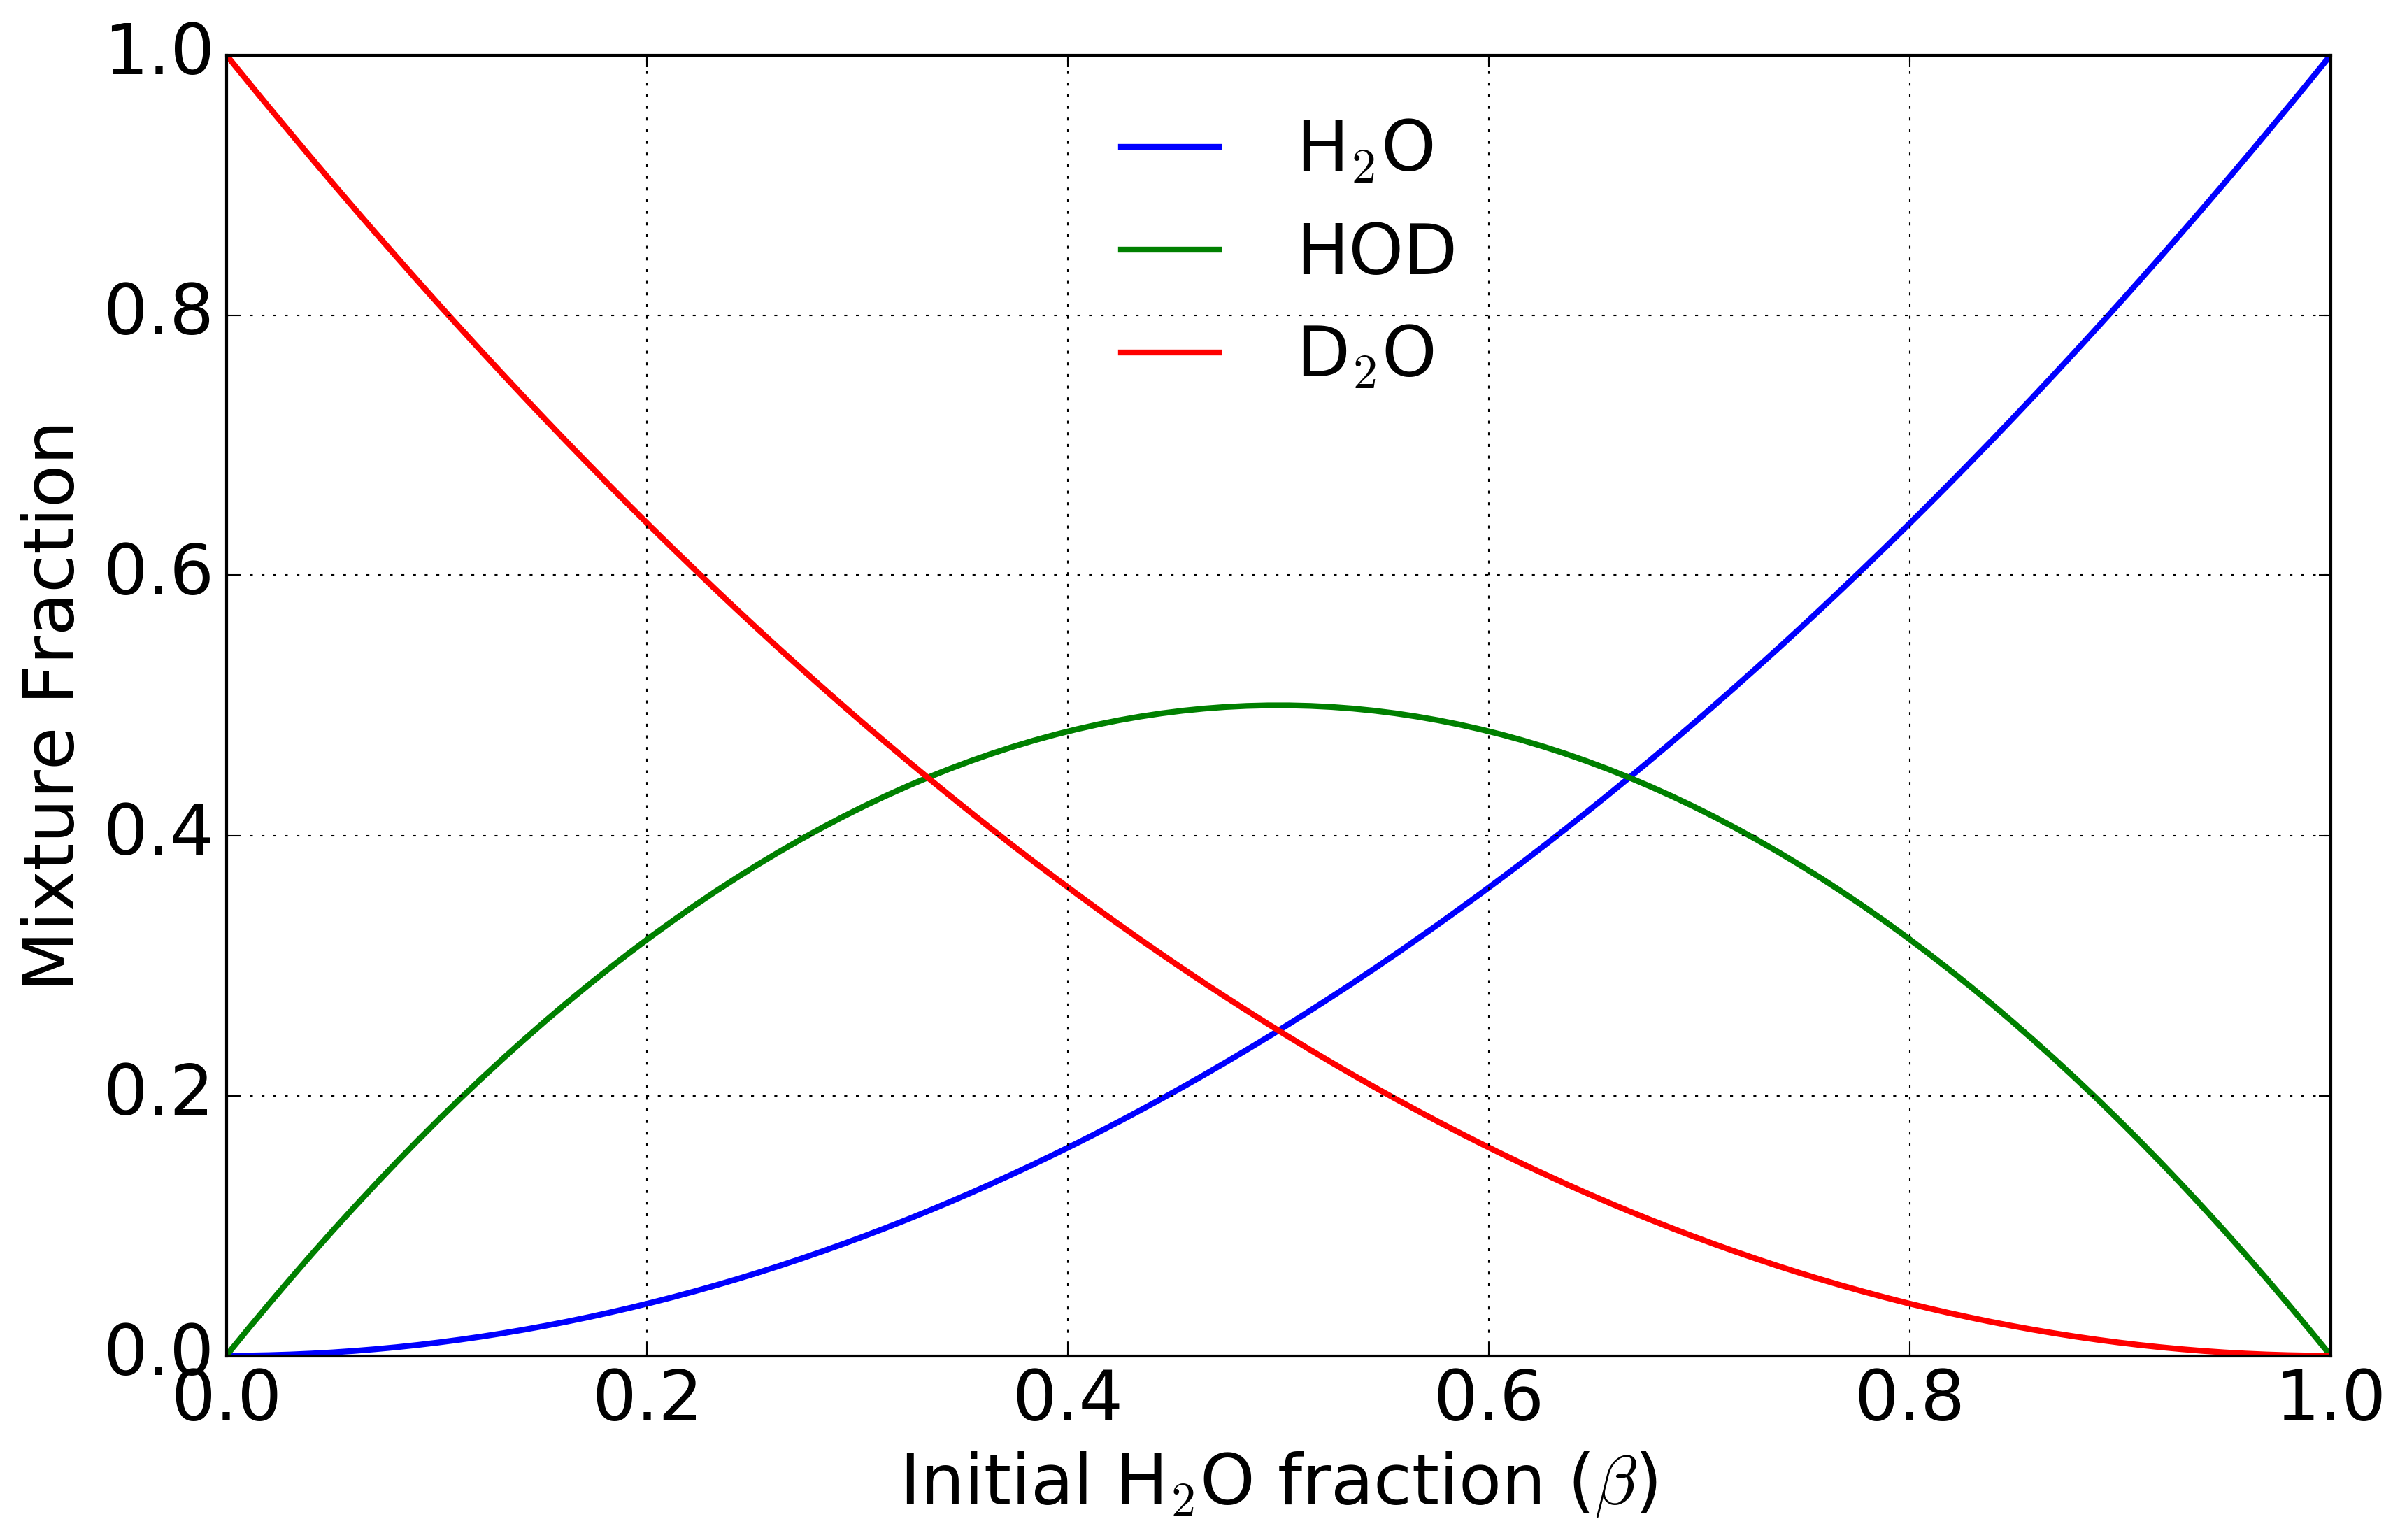
\includegraphics[width=0.8\textwidth]{behod_isotopologues.png}
\caption{}
\end{figure}

Reading water with an RGA causes some known fractionation, where the H$_2$O is broken into its constituents, including OH$^+$ and O$^+$. We expect then to see a lower mass 18 peak than normal, to truly know what the ratios are, we have to calibrate the RGA ourselves.

Possible fractionation pathways:

\begin{align}
P'_{18} = & \alpha P_{H_2O} + \beta (\frac{P_{HOD}}{2}+P_{D_2O}) \\
P'_{19} = & \alpha P_{HOD} \\
P'_{20} = & \alpha P_{D_2O} \\
P'_{17} = & \beta (\frac{P_{HOD}}{2} + P_{H_2O}) \\
P'_{16} = & \gamma (P_{H_2O} + P_{HOD} + P_{D_2O}) \\
1 = & \alpha + \beta + \gamma
\end{align}

By solving this system of equations, we get:

\begin{table}[H]
\centering
\begin{tabular}{l|l|l|l}
Date      & $\alpha$ & $\beta$  & $\gamma$ \\ \hline
8/20/2018 & 0.769 & 0.178 & 0.052 \\ \hline
8/21/2018 & 0.769 & 0.184 & 0.047 \\ \hline
8/22/2018 & 0.767 & 0.193 & 0.040
\end{tabular}
\end{table}

76.8\% of the real value as cited by the RGA program itself; this is also true for HOD and D$_2$O. Of that lost 23.2\%, 18.4\% goes to OH$^+$, but for the isotopogues of HOD and D$_2$O, we would need to consider which mass signal it will add to. No other mode of fractionation will contribute to the other water isotopologue peaks

\begin{align}
P'_1 & = \alpha P_1 + \beta P_3 + \frac{\beta}{2} P_2 \\
P'_2 & = \alpha P_2 \\
P'_3 & = \alpha P_3
\end{align}

Where we let $\alpha = 0.744$ and $\beta=0.256$ per the SRS RGA software. Where P is the real pressure accounting for fractionation, and P' is the raw observed pressure value. Solving for the real pressure, we find:

\begin{align}
P_1 & = \frac{1}{\alpha}\left(P'_1 - \frac{\beta}{\alpha}P'_3 - \frac{\beta}{2\alpha} P'_2\right) \\
P_2 & = \frac{P'_2}{\alpha} \\
P_3 & = \frac{P'_3}{\alpha}
\end{align}

\section{Be$^+$ + HOD branching ratio}

Now that we can characterize the pressures in the chamber more accurately, we then consider the possible reactions between the Be$^+$ and water isotopologues:

\begin{align}
Be^+ + H_2O & \rightarrow BeOH^+ + H \\
Be^+ + HOD & \rightarrow BeOH^+ + H \label{eq: beoh} \\
 & \rightarrow BeOD^+ + H \label{eq: beod} \\
Be^+ + D_2O & \rightarrow BeOD^+ + D
\end{align}

Which can then be written as a system of differential equations.

\begin{align}
\dot{Be}(t) & = -(k_1\rho_1+k_2\rho_2+k_3\rho_3)Be(t) \\
\dot{BeOH}(t) & = (k_1\rho_1+(1-\eta)k_2\rho_2)Be(t) \\
\dot{BeOD}(t) & = (k_3\rho_3+\eta k_2\rho_2)Be(t)
\end{align}

We are interested in reactions \ref{eq: beoh} and \ref{eq: beod} and the ratio between the two ($\eta$), which is not directly found from the ratio of the production rates of the two ions. Since this is a ratio, we don't need to concern ourselves with calculating the density ($\rho$), the RGA pressure is fine.

\begin{align}
\beta \equiv \frac{\dot{BeOD}}{\dot{BeOH}} & = \frac{k_3P_3 + \eta k_2P_2}{k_1P_1 + (1-\eta)k_2P_2} \\
\eta & = \frac{\beta(k_1P_1 + k_2P_2)-k_3P_3}{k_2P_2(1+\beta)}
\end{align}

The theorists found that the statistical value of the reaction is around 3, but with dynamics, tends towards $\frac{\eta}{1-\eta} = 1.7$ or $\eta=0.63$ for Be$^+$(S).

\bibliographystyle{abbrv}
\bibliography{Mendeley}

\end{document}
